\chapter{A combinatorial model for digital elastica shape optimization}
\chaptermark{A combinatorial model for digital elastica}
\label{chapter:digital-elastica}

\daniel{The goal of this chapter is to experimentally validate a model for the elastica energy using multigrid convergent estimators of length and curvature. In~\cref{ch5:sec:continuous-digital-elastica} we introduce the digital elastica and in~\cref{ch5:sec:local-combinatorial-scheme} we present a combinatorial optimization model capable to evolve a shape to another of lower digital elastica energy. In several occasions, the final shape is indeed the optimal one, which confirms the pertinence of using multigrid convergent estimators to optimize geometric-related energies in digital sets. In~\cref{ch5:sec:global-optimization}, we present several attempts to derive a global model to minimize a simplification of the digital elastica and we discuss why they fail.}

%In this chapter we review the elastica energy and some of its properties. Next, we introduce the digital version of the elastica using multigrid convergent estimators of length and curvature. We present a combinatorial optimization model capable to evolve a shape to another of lower digital elastica energy. In several occasions, the final shape is indeed the optimal one, which confirms the pertinence of using multigrid convergent estimators to optimize geometric-related energies in digital sets. Finally, we present several attempts to derive a global model to minimize a simplification of the digital elastica and we discuss why they fail.

\section{Digital elastica}
\label{ch5:sec:continuous-digital-elastica}
	The elastica energy of parameters $\Theta=(\alpha \geq 0, \beta \geq 0)$ for some Euclidean shape $S \subset \mathbb{R}^2$ is defined as
	\begin{align*}
	E_{\Theta}(S) &= \int_{\partial S}{ \alpha + \beta \kappa(s)^2 ds}.
	\end{align*}
Similarly, the digital elastica $\hat{E}_{\Theta}$ of some digitization $D_h(S)$ of $S$ is defined as
	\begin{align}
	\hat{E}_{\Theta}( D_h(S) ) = \sum_{\dot{\vec{e}} \in \partial_h S}{ \hat{s}( \dot{\vec{e}})\left(\; \alpha + \beta \hat{\kappa}^2(D_h(S),\dot{\vec{e}},h) \; \right)},
	\label{ch5:digital-elastica}
	\end{align}
where $\dot{\vec{e}}$ denotes the center of the linel $\vec{e}$ \daniel{and the estimators of length $\hat{s}$ and curvature $\hat{\kappa}$ are multigrid convergent}. In the
expression above, we will substitute an arbitrary subset $\Ds$ of
$\mathbb{Z}^2$ to $D_h(S)$ since the continuous shape $S$ is unknown.
In the following we omit the grid step $h$ to simplify expressions
(or, putting it differently, we assume that the shape of interest is
rescaled by $1/h$ and we set $h=1$). 

 In the next section, we describe a combinatorial scheme whose aim is to optimize the digital elastica energy~\cref{ch5:digital-elastica}.
% that permit us to find the minimum digital shape with respect the digital elastica energy for some neighborhood of shapes of $\Ds$. 

\section{Local combinatorial scheme}
\label{ch5:sec:local-combinatorial-scheme}

Given a digital shape $\Ds^{(0)}$ we describe a process that generates a
sequence $\Ds^{(i)}$ of shapes with non-increasing elastica energy. The
idea is to define a neighborhood of shapes $\mathcal{N}^{(i)}$ to the
shape $\Ds^{(i)}$ and choose the element of $\mathcal{N}^{(i)}$ with
lowest energy.  

Let $\Ds$ be a $2$-dimensional digital shape embedded in a domain $\Omega \subset \mathbb{Z}^2$. We adopt the cellular-grid model to represent $\Ds$, i.e., pixels and its lower dimensional counterparts, linels and pointels, are part of $\Ds$ (see~\cref{ch5:fig:cellular-grid-model}). In particular, we denote by $\partial \Ds$ the topological boundary of $\Ds$, i.e., the connected sequence of linels such that for each linel we have one of its incident pixels in $\Ds$ and the other not in $\Ds$.

\begin{figure}[]
	\center
	\subfloat[\label{ch5:fig:flower-shape}]{%
	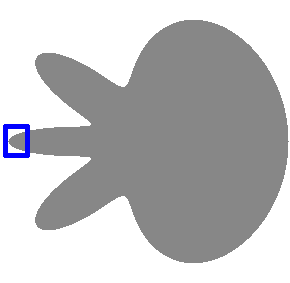
\includegraphics[scale=1.8]{figures/chapter5/cellular-grid/flower.png}
	}\hspace{20pt}%
	\subfloat[\label{ch5:fig:cellular-grid-model}]{%	
	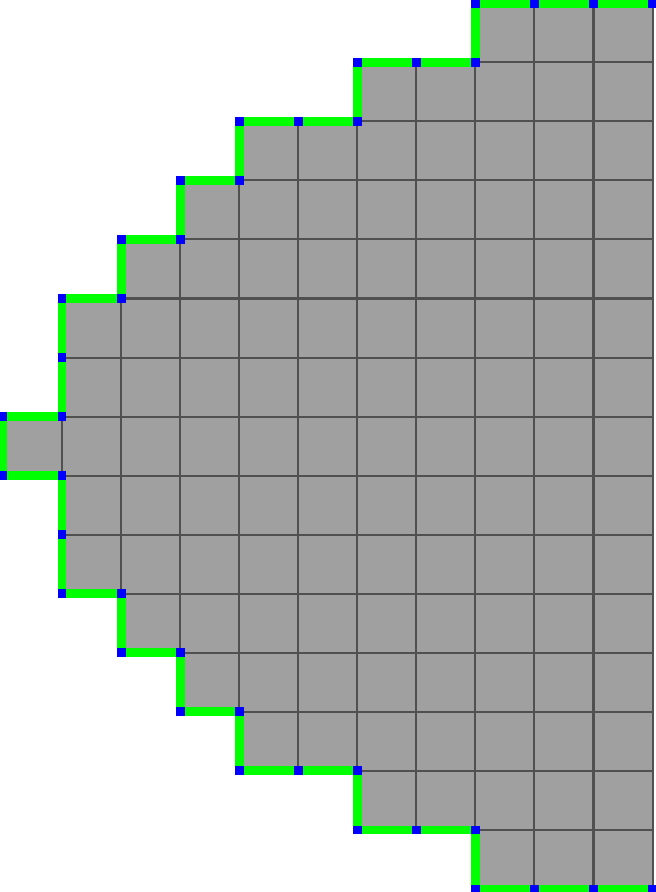
\includegraphics[scale=0.27]{figures/chapter5/cellular-grid/cellular-grid-illustration.pdf}
	}\hspace{20pt}%
	\subfloat[\label{ch5:fig:ring-set}]{%
	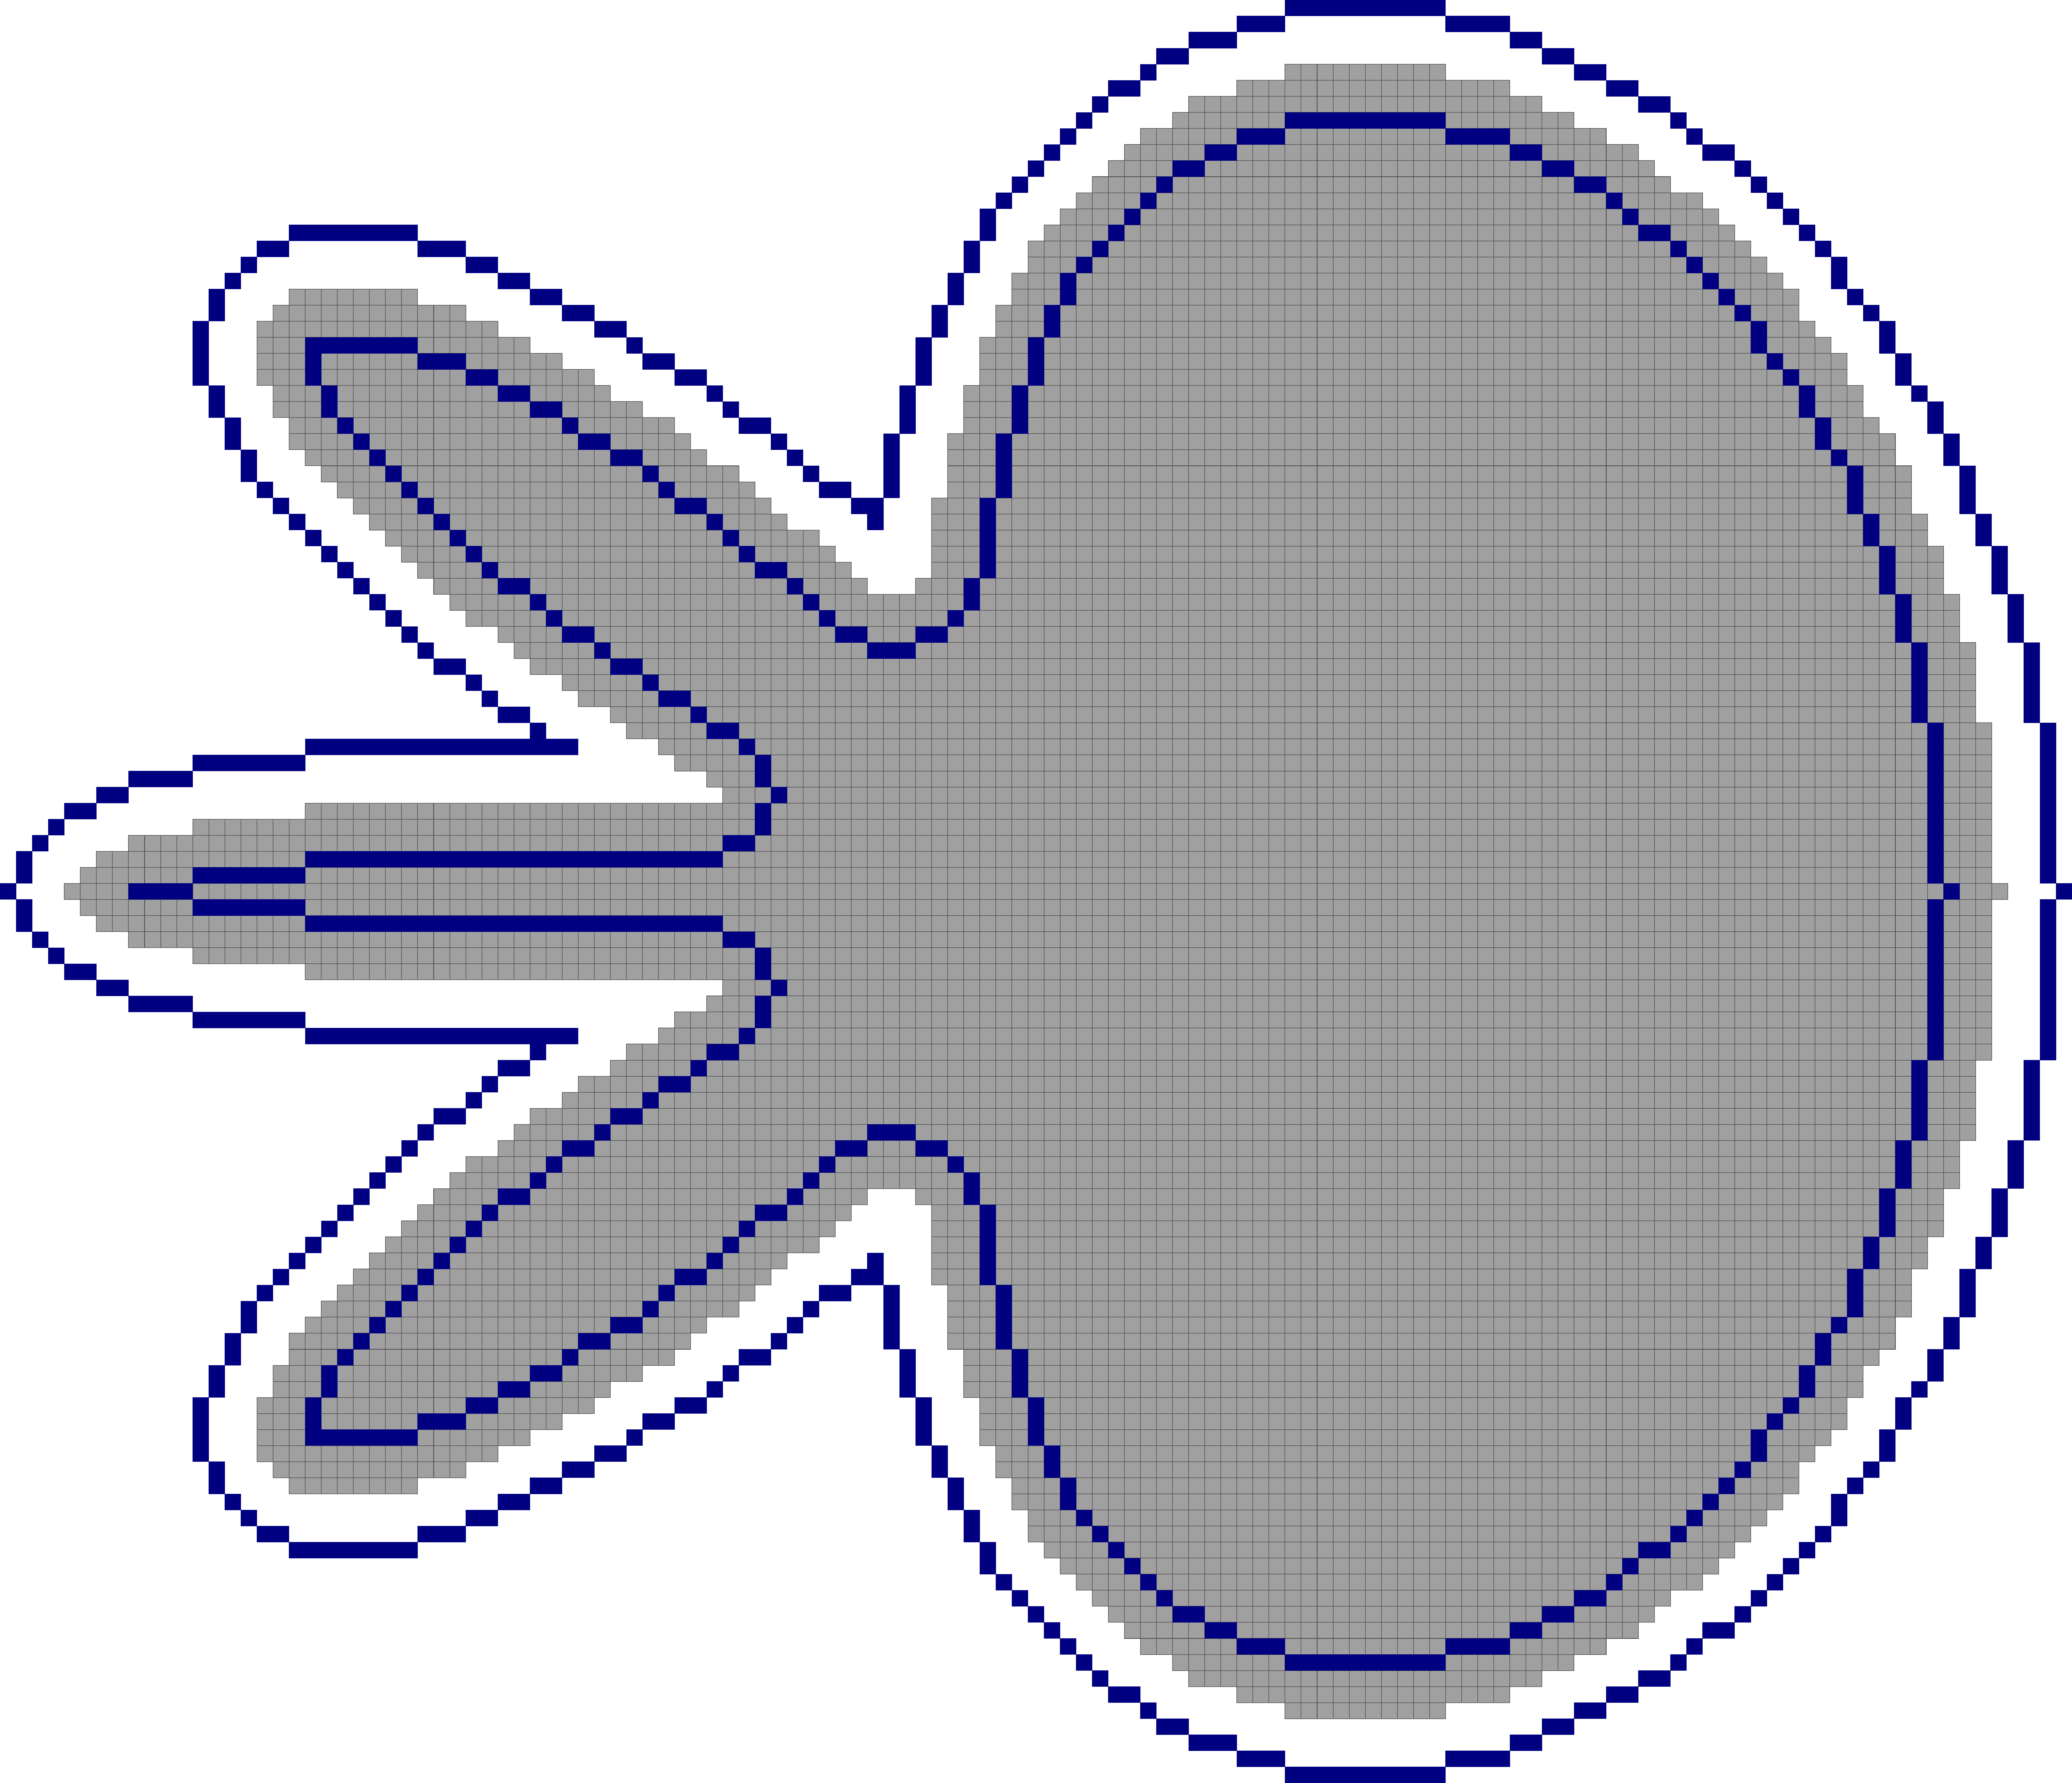
\includegraphics[scale=0.035]{figures/chapter5/m-ring/L4-nodt.pdf}
	}
	\caption{\daniel{\textbf{Cellular grid model and $m$-ring set.}}The flower shape in figure (a) and the cellular-grid model representation in (b) of the \daniel{blue} bounded  rectangle region \daniel{in (a)}. In figure (b), pixels are colored in gray, linels in green and pointels in blue. In figure (c), the blue pixels denotes a $3$-ring set.}
\end{figure}

Let $d_{\Ds}:\Omega \rightarrow \mathbb{R}$ be the signed Euclidean distance transformation with respect to shape $\Ds$. The value $d_{\Ds}(p)$ gives the Euclidean distance between $p \notin \Ds$ and the closest pixel in $\Ds$. For points $p \in \Ds$, $d_{\Ds}(p)$ gives the negative of the distance between $p$ and the closest pixel not in $\Ds$.
\begin{definition}{Inner pixel boundary}

Given a digital shape $\Ds$ embedded in a domain $\Omega$, we define its inner pixel boundary set $I(\Ds)$ as
\begin{align*}
	I(\Ds) := \left\{ \: p \; | \; p \in \Ds, |\mathcal{N}_4(x) \cap \Ds|<4 \: \right\},
\end{align*}
where $\mathcal{N}_4(p)$ denotes the $4$-adjacent neighbor set of $p$ (without $p$). 
\end{definition}
\begin{definition}{m-Ring Set}
Given a digital shape $\Ds \in\Omega$, its signed distance transformation $d_{\Ds}$ and natural number \daniel{$m \geq 0$} %$m \neq 0$, 
the {\em $m$-ring set of $\Ds$} is defined as
\begin{align*}
	R_m(\Ds) &:= L_m \cup L_{-m},
\end{align*}
where
\begin{align*}
	L_m(\Ds) &:= \left\{ \quad \begin{array}{rc}
		\daniel{I(D)}, & \daniel{m=0}\\
		\left\{ p \in \Omega \; | \; m-1 < d_{\Ds}(p) \leq m \right\}, &  m>0\\
		\left\{ p \in \Omega \; | \; m+1 > d_{\Ds}(p) \geq m \right\}, &  m<0
		\end{array} \right.
\end{align*}
\end{definition}
\daniel{Thus, the $m$-ring is composed out of two sets of pixels with positive and negative distances to the shape $D$ if $m > 0$~(see~\cref{ch5:fig:ring-set}), and equal to the inner pixel boundary in the case $m=0$.} Consider the following set of neighbor candidates to $\Ds$:
\begin{align*}
\{ Q \; | \; Q \subset R_1(\Ds) \cup \Ds \; \text{and} \; \text{$Q$ is connected} \}.
\end{align*}
Such set can be extremely large and its complete exhaustion is prohibitively expensive.  Instead, we are going to use a subset of it.
\begin{definition}{$n$-neighborhood}

	Given a digital shape $\Ds \subset \Omega$, its $n$-neigh\-bor\-hood $\mathcal{N}_n(\Ds)$ is defined as the set of digital shapes that can be built from $\Ds$ by adding or removing a sequence of $k \in [0,n]$ connected pixels in $R_1(\Ds)$.

\end{definition}

\begin{figure}
\center
\subfloat{
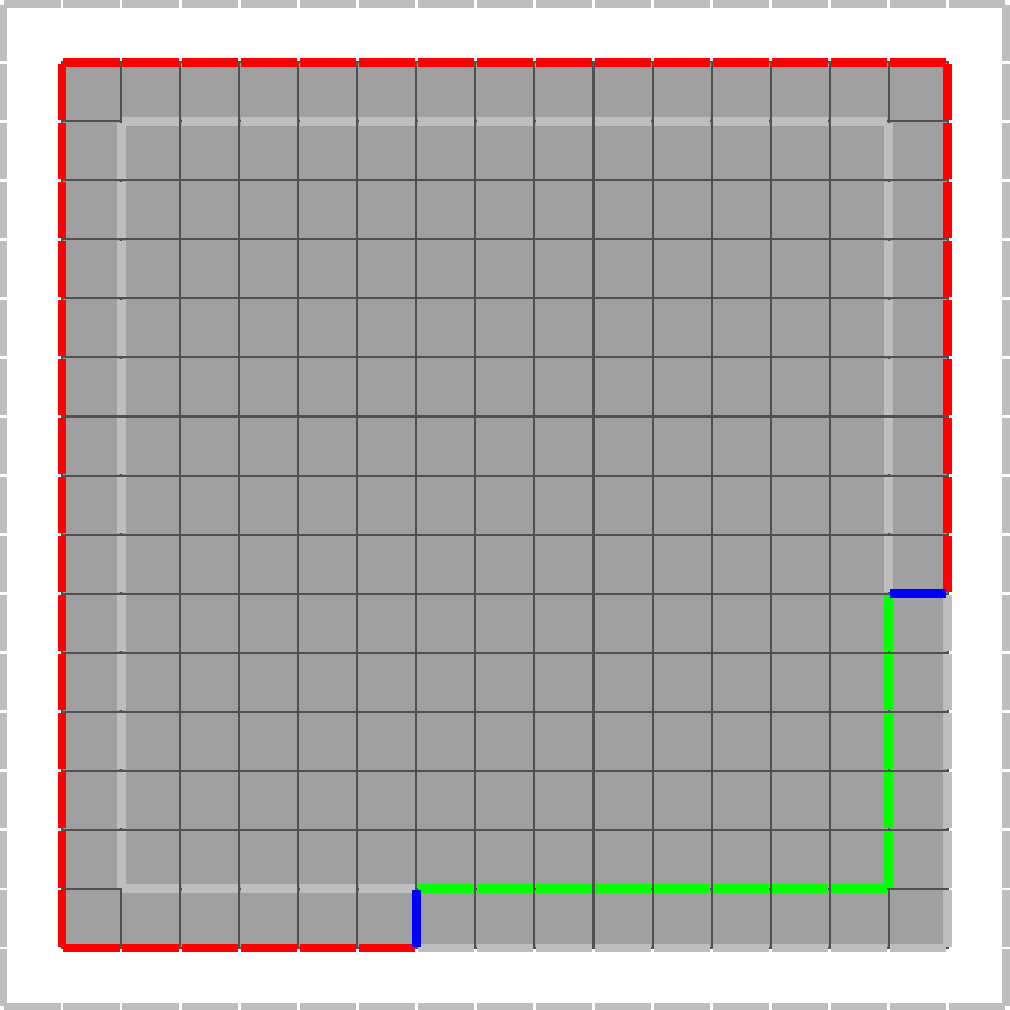
\includegraphics[scale=0.25]{figures/chapter5/gcurves/gc/main-inner.pdf}
}\hspace{1em}%
\subfloat{
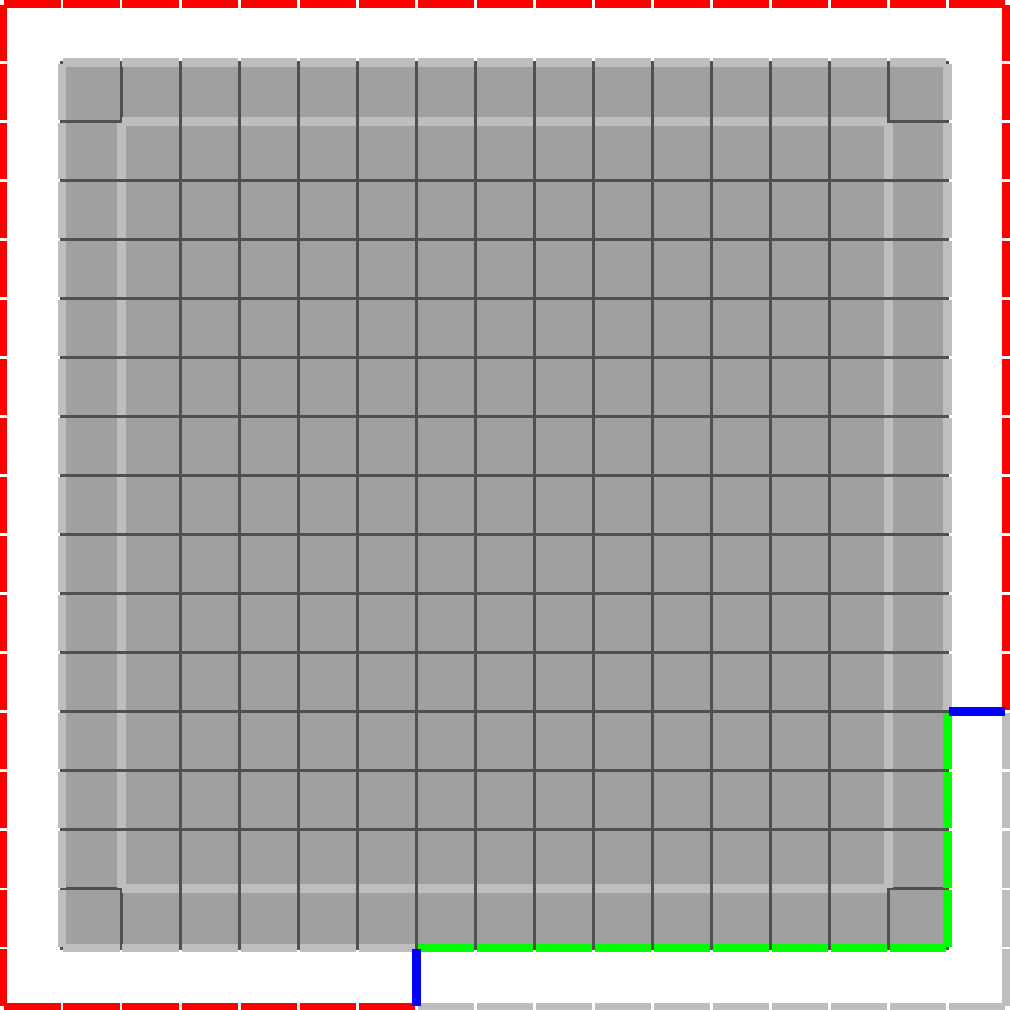
\includegraphics[scale=0.25]{figures/chapter5/gcurves/gc/main-outer.pdf}
}
\caption{\daniel{\textbf{$12$-Neighborhood of the square shape.}The black linels mark the digital contour of the original shape and the gray linels mark the $1$-ring. In the left, a member of $\mathcal{N}_{12}$ in which the red pixels were removed; and in the right a member of $\mathcal{N}_{12}$ in which the yellow pixels were added.} }
\label{ch5:fig:n12-neighborhood}
\end{figure}


\daniel{In~\cref{ch5:fig:n12-neighborhood} it is shown two members of the $\mathcal{N}_{12}$ neighborhood.} At first glance, we may be tempted to set the local-search neighborhood at the $k$-th iteration as the union of all $n$-neighborhood for $1<n<|\partial \Ds^{(k)}|$. However, that is often unnecessary and time consuming, as the greatest reduction in digital elastica for a member of $\mathcal{N}_n$ is likely very close to the greatest reduction for a member of $\mathcal{N}_{n-1}$. Moreover, we can improve running time by implementing a multiscale approach, i.e., we look for reductions in digital elastica for larger values of $n$ first, and in case of a negative answer we refine our search by choosing a smaller $n$.

The \emph{LocalSearch}~\cref{ch5:alg:local-search} describes the local combinatorial process and is suitable for \daniel{any combination of multigrid convergent estimators of perimeter and curvature. In our experiments, we set the $\lambda$-MST~\cite{lachaud07tangent} to estimate elementary length and perimeter. We compare our results for two curvature estimators: the MDCA~\cite{roussillon11mdca} and the integral invariant (II-$r$) estimator~\cite{coeurjolly13integral} ($r$ denoting the radius of the estimation ball).} 

% type of digital estimator. To estimate length we use MDSS and to estimate curvature we execute~\cref{alg:local-search} with the MDCA and II-$r$ estimators  to solve the free and constrained elastica problems. 
	


\begin{algorithm}
 \SetKwData{It}{k}
 \SetKwData{MIt}{maxIt}
 \SetKwData{Delta}{delta}
 \SetKwData{Best}{best} 
 \SetKwInOut{Input}{input}\SetKwInOut{Output}{output}
 \SetKwComment{comment}{//}{}
 
 \Input{A digital set $\Ds$; weight coefficients $\Theta=(\alpha , \beta)$; the maximum number of iterations \MIt}
 \BlankLine
 $t \longleftarrow 1$ \tcp*[l]{multiscale level}
 $k \longleftarrow 0$	\tcp*[l]{current iteration}
 $\Ds^{(0)} \longleftarrow \Ds$\;
 \While{ \It $<$ \MIt \bf{and} $t < \log_2{|\partial \Ds^{(k)}|}$ }
 { 	
%	$M^{(k,t)}  \longleftarrow |\partial \Ds^{(k)}|/2^t$  	\tcp*[l]{Maximum $n$-neighborhood value.}
%	
%	$J \longleftarrow \{ j \cdot \frac{M^{(k,t)}}{nc} \; | \; 1 \leq j \leq nc \} $\;
%	
%	$\displaystyle \mathcal{N}^{(k,t)} \longleftarrow \displaystyle \Cup_{J}{\mathcal{N}_{j}(\Ds^{(k)})}$\;

	$n  \longleftarrow |\partial \Ds^{(k)}|/2^t$  	\tcp*[l]{Maximum $n$-neighborhood value.}
	
	$\displaystyle \mathcal{N}^{(k,t)} \longleftarrow \displaystyle \mathcal{N}_{n}(\Ds^{(k)})$\;
	
	\BlankLine
	
	\comment{Find neighbor shape with lowest energy.} 
	$Q^{\star} \longleftarrow D^{(k-1)}$\;
  	\For{$ Q \in \mathcal{N}^{(k,t)} $}
	{
		\If{ $\hat{E}_{\Theta}(Q)$ $<$ $\hat{E}_{\Theta}(Q^\star)$ }
		{
			$Q^\star \longleftarrow Q$\; 
		}	
	}
	\BlankLine
	

	\Delta $\longleftarrow$ $\hat{E}_{\Theta}(\Ds^{(k-1)}) - \hat{E}_{\Theta}(\Ds^{(k)})$\;	
	
	\If{ \Delta $\leq 0$ } 
	{
		\comment{Better solution not found. Refine the scale.}
		$t \longleftarrow t+1$ 
	}		
	\Else 
	{ 
		\comment{Better solution found. Set $D^{(k)}$ and reset to highest scale.}
		$t \longleftarrow 1$\;	
		$\Ds^{(k)} \longleftarrow Q^\star$\;
		\It $\longleftarrow$ \It $+1$\;		
	}
	
 }
 \caption{LocalSearch algorithm for elastica minimization.}
  \label{ch5:alg:local-search} 
\end{algorithm}

\daniel{
\section{Experimental results}
We study the behaviour of~\cref{ch5:alg:local-search} in two problem configurations. 

\begin{itemize}
	\item[]{ \textbf{Free elastica.} The digital elastica~\cref{ch5:digital-elastica} is optimized without any constraint. }
	\item[]{ \textbf{Constrained elastica.} We force pixels to be present in the final shape or we impose an orientation in the endpoints of a segment of the digital contour.}	
\end{itemize}
}

\subsection{Free elastica}
\label{ch5:subsec:free-digital-elastica}
\daniel{
As observed in~\cref{ch3:sec:elastica-curve}, the closed planar curve that minimizes the free elastica is the circumference of a disk of radius $(\beta/\alpha)^{0.5}$
\begin{align*}
	\partial B_{(\beta/\alpha)^{0.5}} = \argmin_C \int_{C}{ (\alpha + \beta \kappa^2)ds}.
\end{align*}
}
%We study the performance of~
%In the free digital elastica energy we optimize~\cref{ch5:digital-elastica} without any constraint. We observe that for $\alpha=0, \beta >0$ the elastica becomes the integration of the squared curvature  along the shape contour which has the ball of infinite radius as its minimizer. For $\alpha > 0, \beta=0$, minimize elastica becomes minimize perimeter (curvature flow). It is easy to see that for $\alpha, \beta > 0$, the optimal shape for the elastica is a disk of radius $r$. We can easily find the value of $r$.
%\begin{align*}
%	\frac{d}{dr}\big( \int_{\partial B(r)}{ (\alpha + \beta \kappa ^2) ds} \big ) &= 0\\
%	\frac{d}{dr}\big( \alpha 2\pi r + \beta2\pi/r \big) &= 0\\
%	r &= \left(\frac{\beta}{\alpha}\right)^{1/2}.
%\end{align*}  
%%
%Therefore, the optimal shape for the free digital elastica is a digital disk of finite radius $(\beta/\alpha)^{1/2}$.
%
%
In~\cref{fig:local-comb-estimators-plots-lp001} we present the digital elastica evolution for parameters $\alpha=0.01, \beta=1$ and \daniel{four} different curvature estimators in three different scales. The shapes evolution using the II-$5$ estimator are shown in~\cref{fig:local-comb-ii5-results}. We observe that both II-$5$ and II-$10$ evolve the shapes to disks of radius close to the optimum value of $10$. The II-$3$ estimator stops prematurely at a local optimum due its limited sensibility compared to II-$5$ or II-$10$, while MDCA encounters some difficulties to evolve in a high resolution setting and it also stops at some local minimum. In fact, the MDCA estimator, although with higher convergence speed, is more sensitive to noise than II, as illustrated in~\cref{fig:mdca-sensitivity}. Nonetheless, the results can be improved by using a larger neighborhood, as illustrates~\cref{fig:mdca-larger-neighborhood}.



We have executed the same experiments for different parameters $\alpha$ to confirm the effectiveness of our approach. We observe that the plots for $\alpha=0.001$ in~\cref{fig:local-comb-estimators-plots-lp0001} follows a pattern similar to those in~\cref{fig:local-comb-estimators-plots-lp001} for $\alpha=0.01$. In particular, the remarks for the II-$3$ and MDCA estimator are the same. Further, we point out that II-$5$ values are slightly farther from the optimum for $\alpha=0.001$. The reason being that the shapes evolve to a ball of higher radius compared to the case $\alpha=0.01$. At some point of the evolution for $\alpha=0.001$, the sensibility of II-$5$ is not sufficient to escape from local minimum. We remark that the adoption of an automatic selection of the estimation ball radius may attenuate this problem.



\begin{figure}[]
\center
\subfloat{
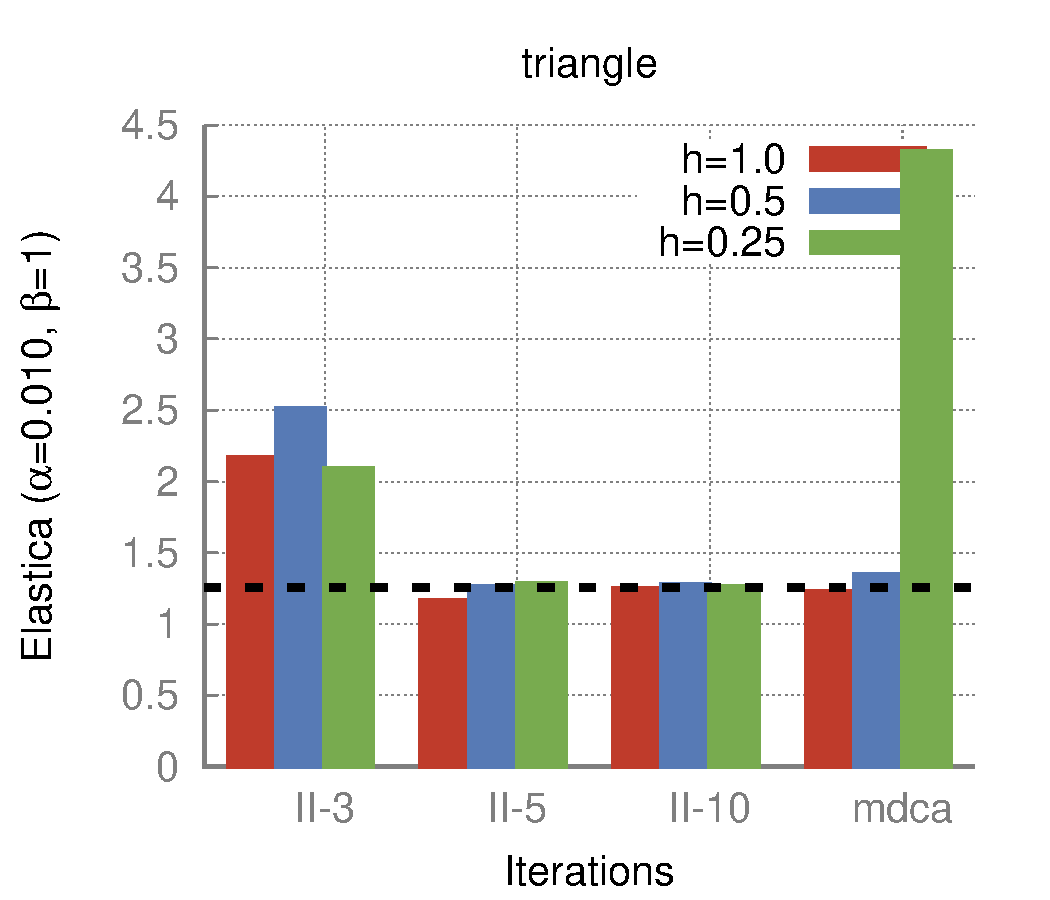
\includegraphics[scale=0.4]{figures/chapter5/flow/plots/bars/length_pen_0.01000/triangle.pdf}
}\hspace{0.25em}%
\subfloat{
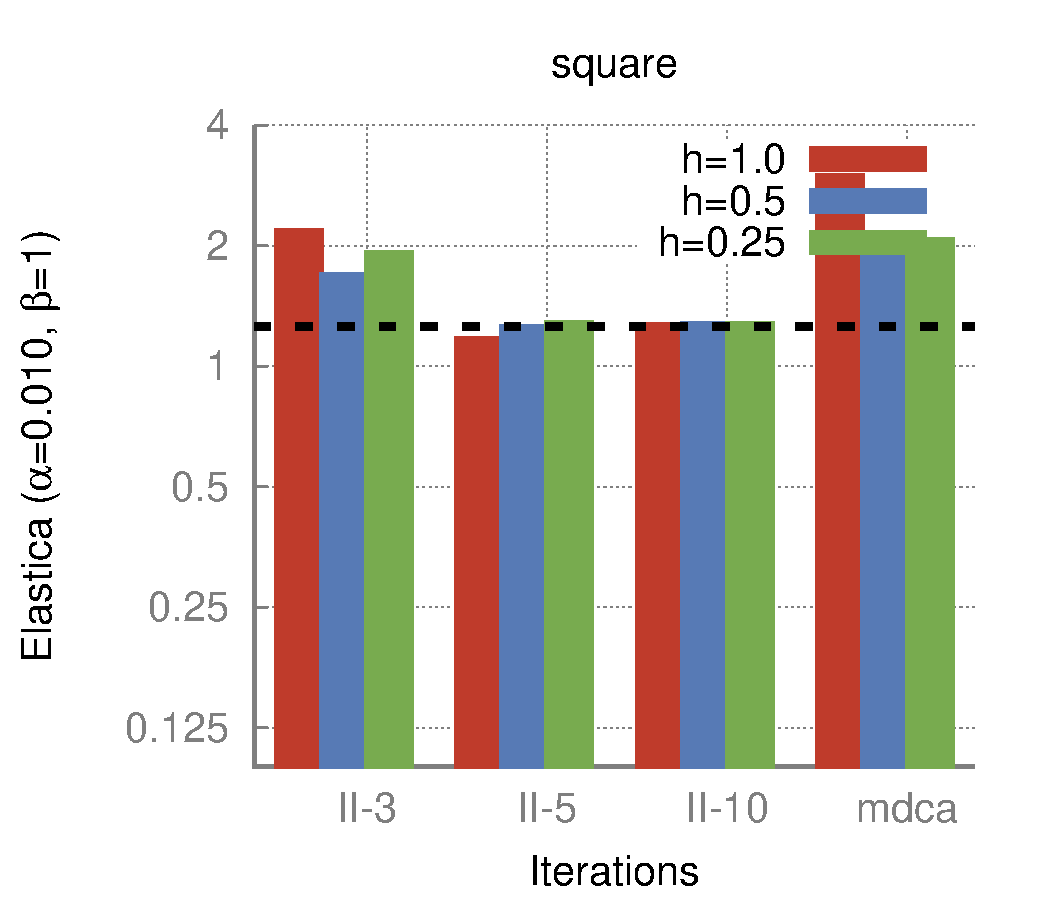
\includegraphics[scale=0.4]{figures/chapter5/flow/plots/bars/length_pen_0.01000/square.pdf}
}\hspace{0.25em}%
\subfloat{
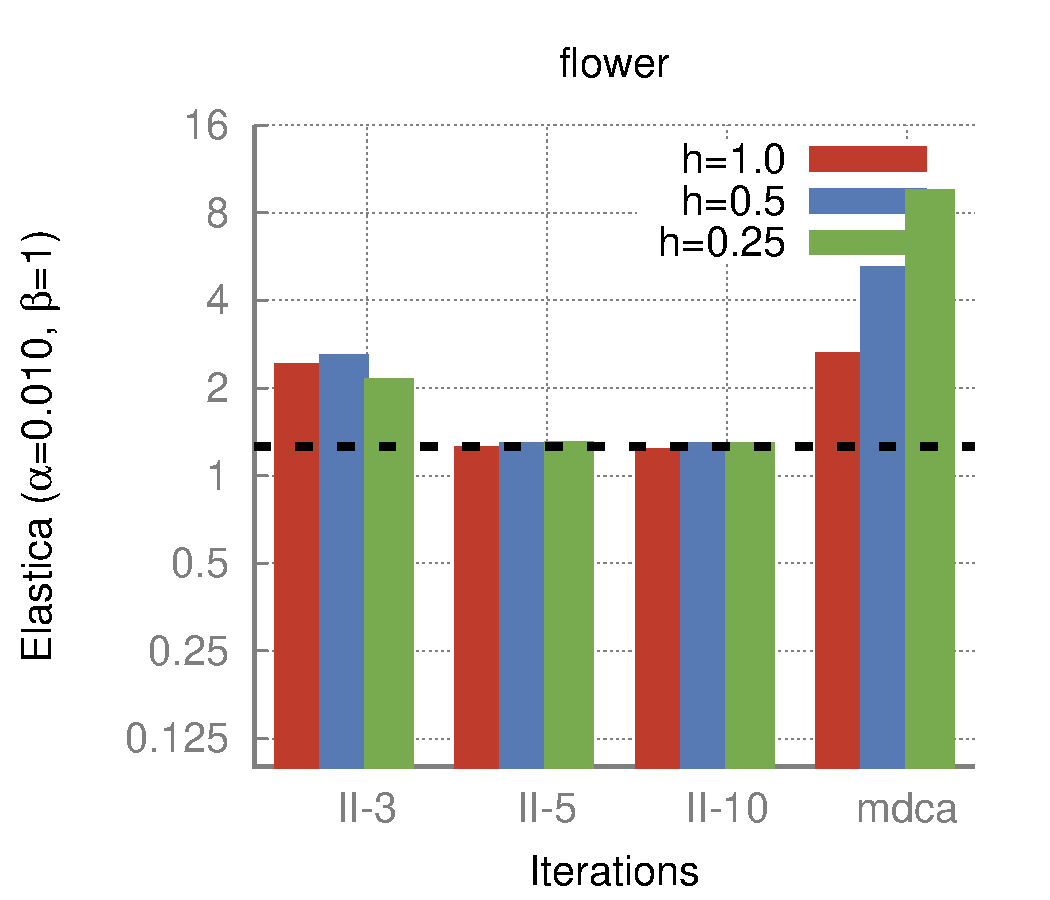
\includegraphics[scale=0.4]{figures/chapter5/flow/plots/bars/length_pen_0.01000/flower.pdf}
}\hspace{0.25em}%
\subfloat{
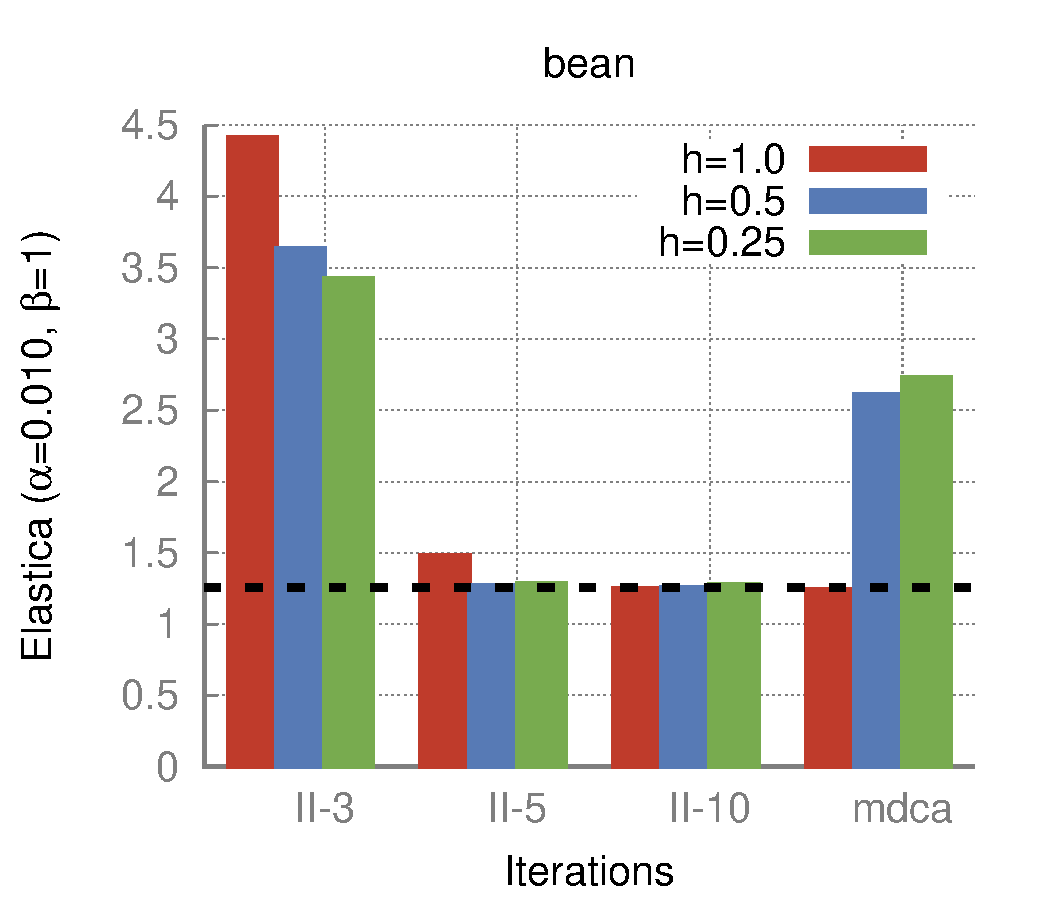
\includegraphics[scale=0.4]{figures/chapter5/flow/plots/bars/length_pen_0.01000/bean.pdf}
}\hspace{0.25em}%
\subfloat{
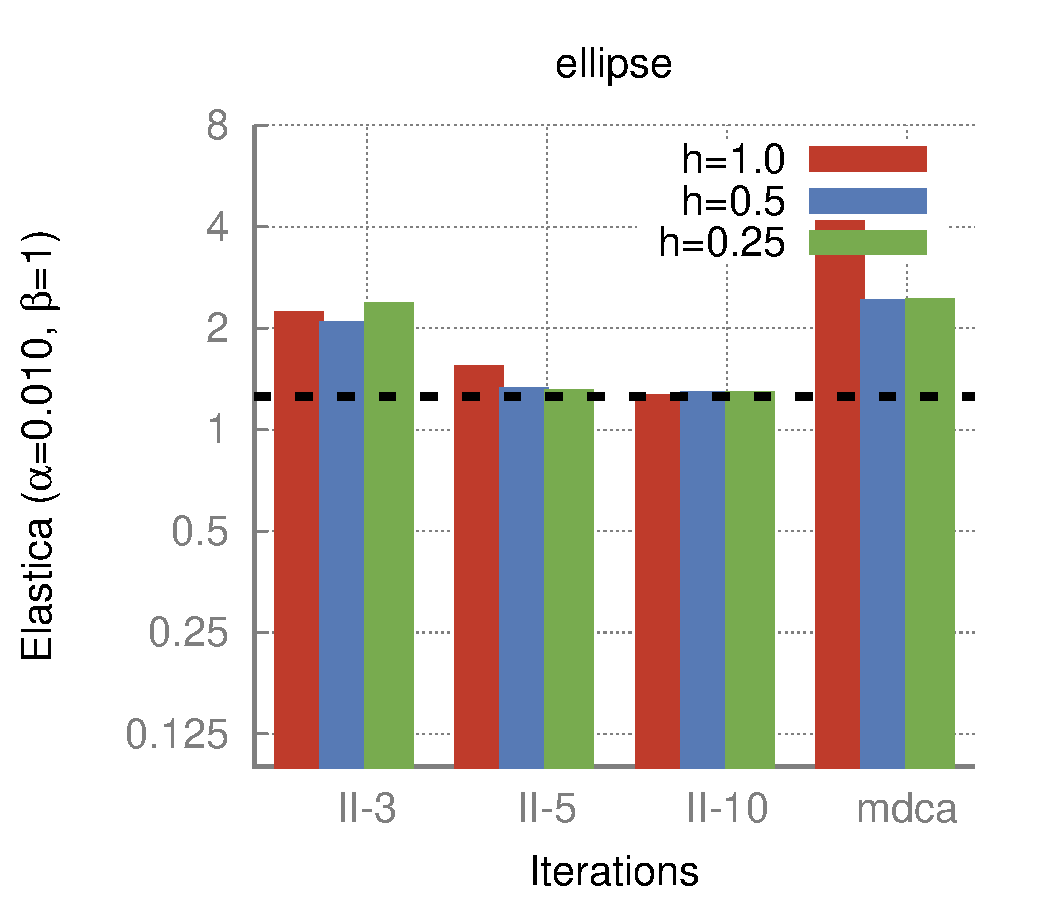
\includegraphics[scale=0.4]{figures/chapter5/flow/plots/bars/length_pen_0.01000/ellipse.pdf}
}\hspace{0.25em}%
\subfloat{
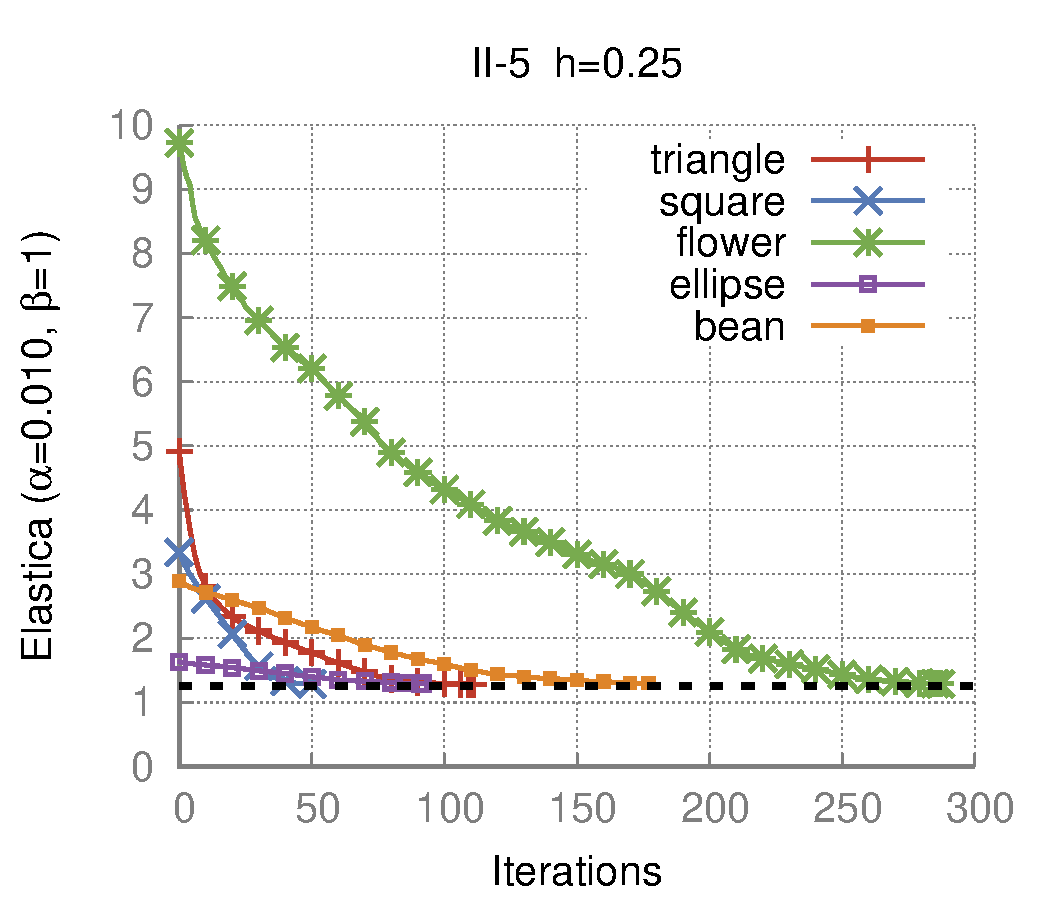
\includegraphics[scale=0.4]{figures/chapter5/flow/plots/summary/lp_0.01/summary-ii5.pdf}
}%
\caption{\daniel{\textbf{Free elastica evolution plots for ($\mathbf{\alpha=0.01, \beta=1}$).}}Minimum value attained for the digial elastica  in comparison with the global optimum (dashed line) for different curvature estimators and in different scales. The last figure summarizes the digital elastica evolution value for all shapes \daniel{using the II-$5$ estimator and} grid step $h=0.25$.}
\label{fig:local-comb-estimators-plots-lp001}
\end{figure}

\begin{figure}[]
\center
\subfloat{
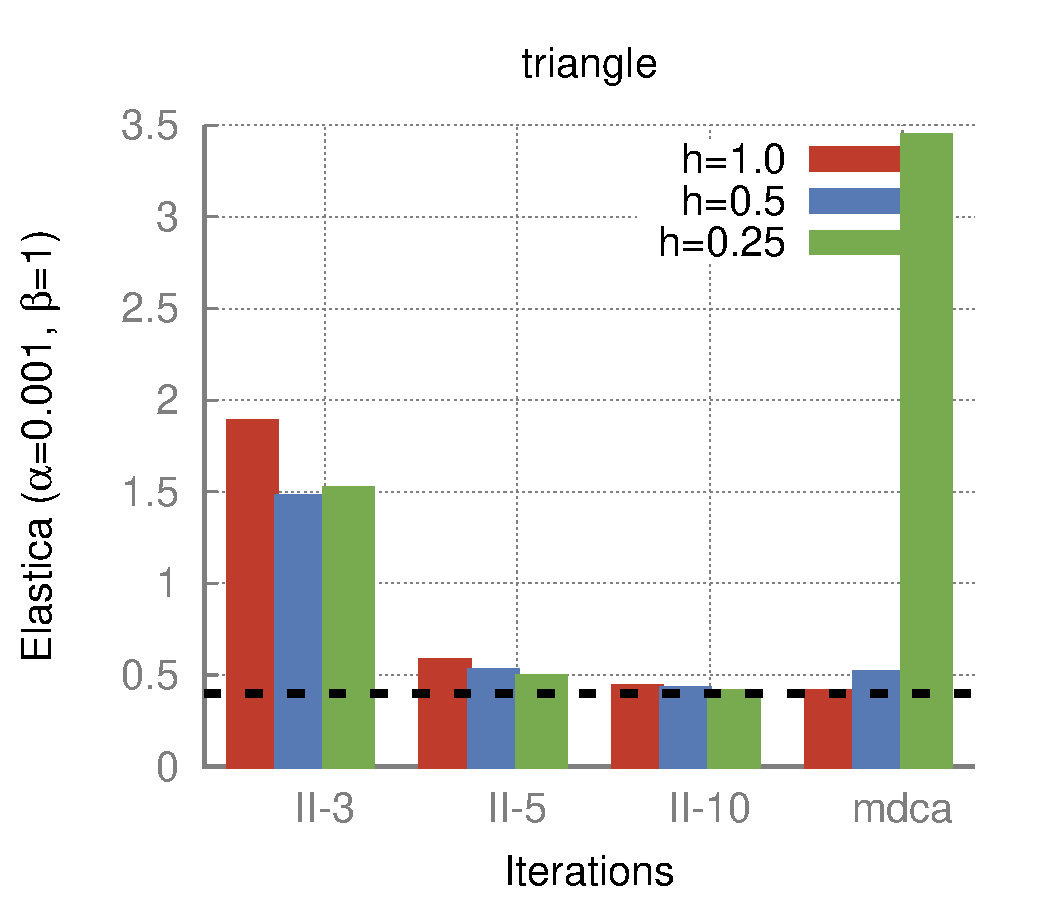
\includegraphics[scale=0.4]{figures/chapter5/flow/plots/bars/length_pen_0.00100/triangle.pdf}
}\hspace{0.25em}%
\subfloat{
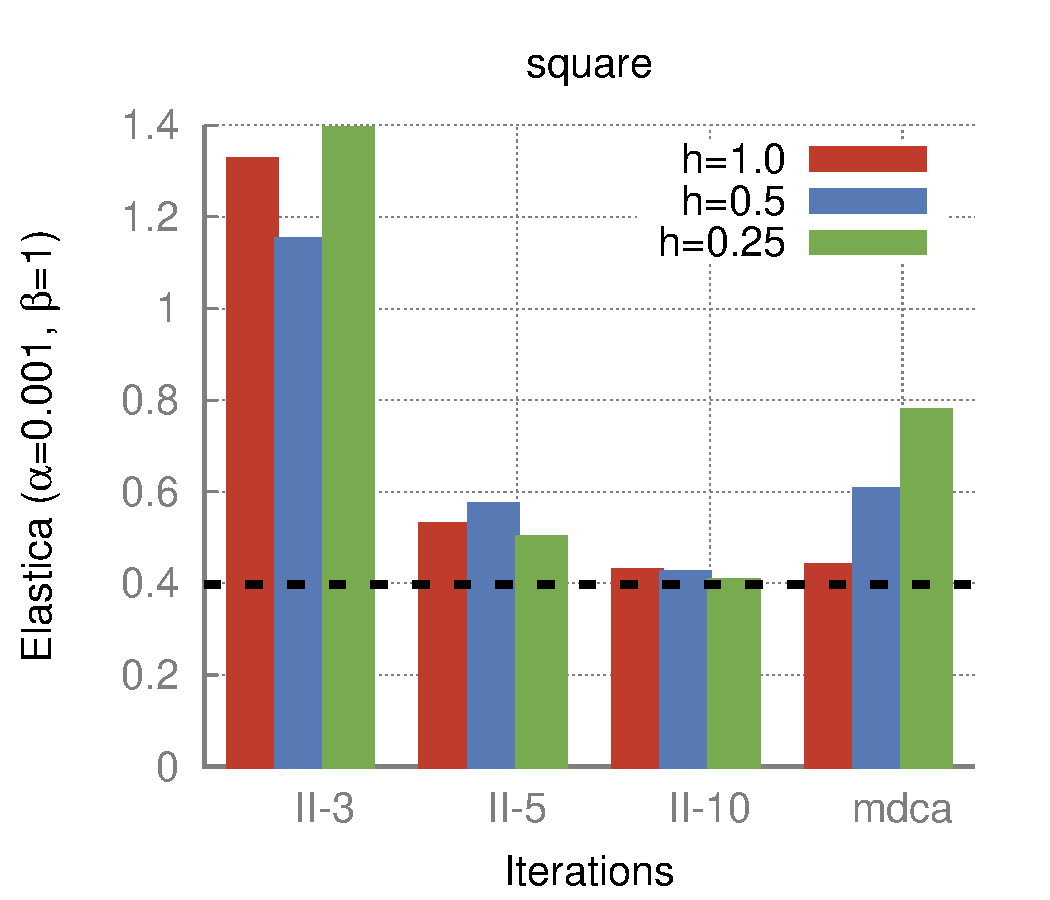
\includegraphics[scale=0.4]{figures/chapter5/flow/plots/bars/length_pen_0.00100/square.pdf}
}\hspace{0.25em}%
\subfloat{
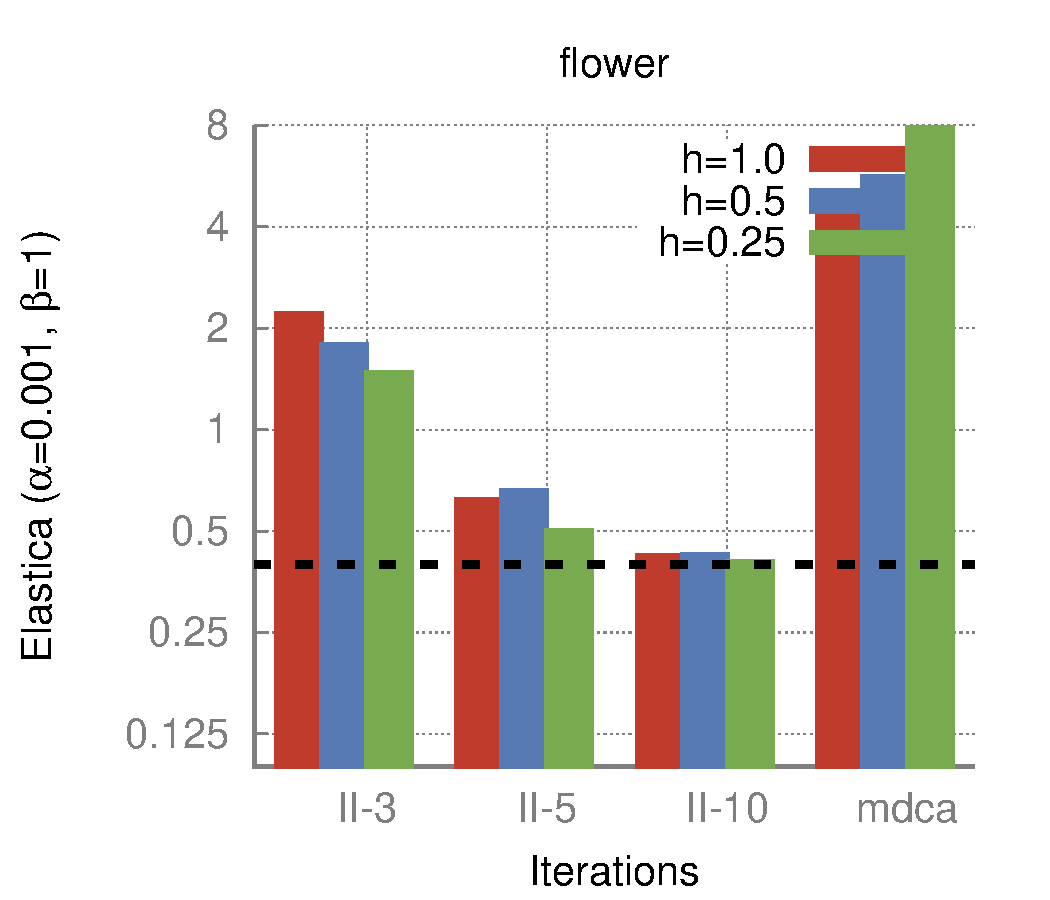
\includegraphics[scale=0.4]{figures/chapter5/flow/plots/bars/length_pen_0.00100/flower.pdf}
}\hspace{0.25em}%
\subfloat{
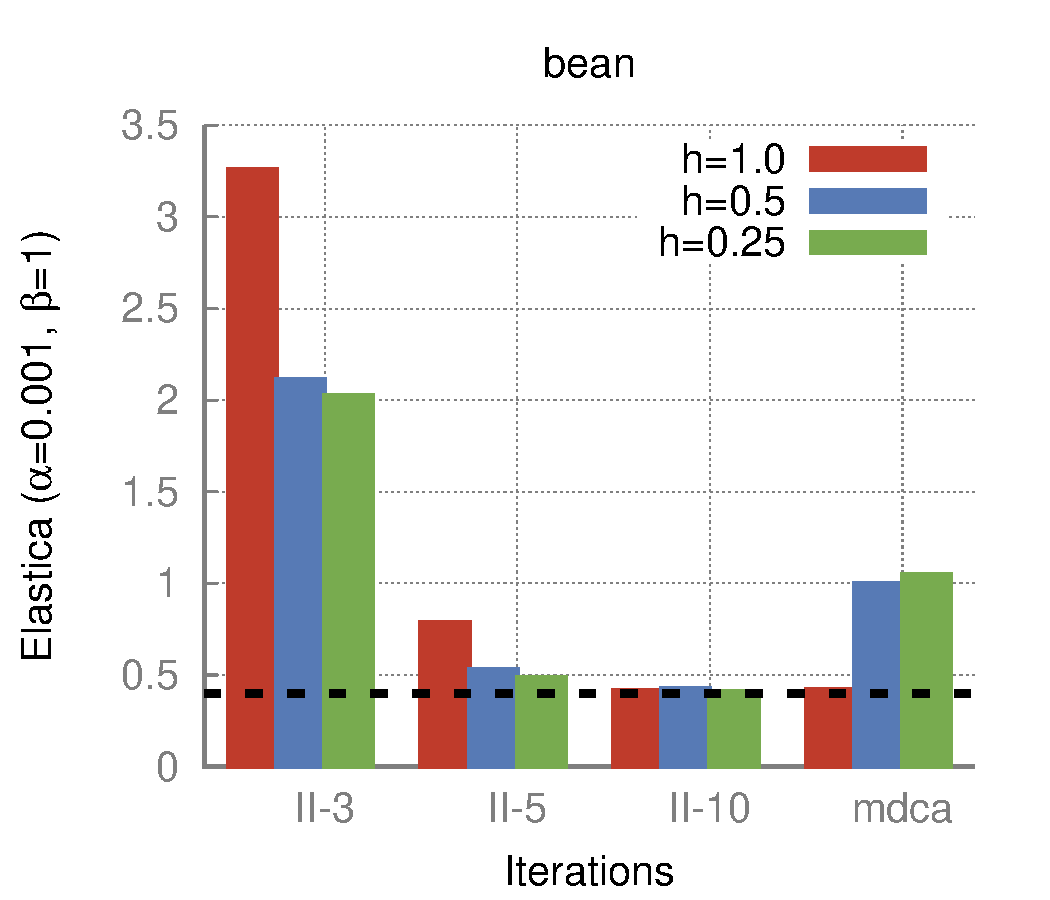
\includegraphics[scale=0.4]{figures/chapter5/flow/plots/bars/length_pen_0.00100/bean.pdf}
}\hspace{0.25em}%
\subfloat{
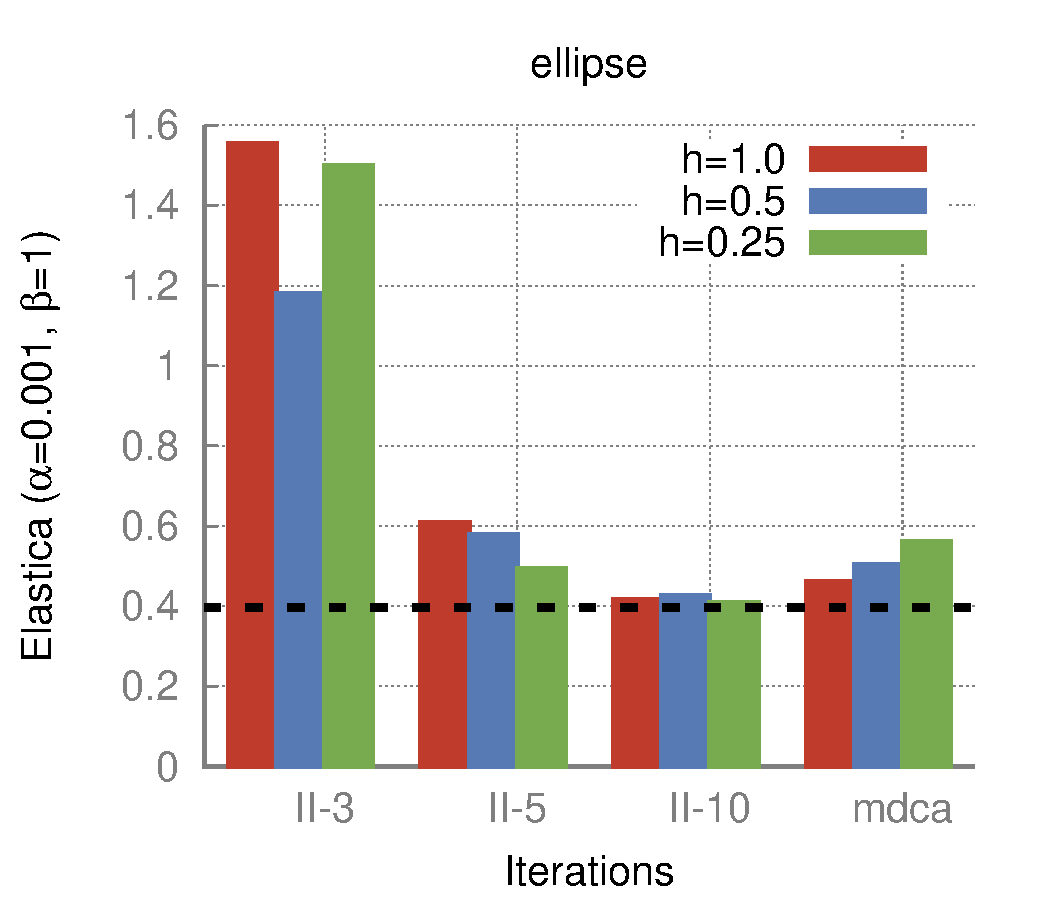
\includegraphics[scale=0.4]{figures/chapter5/flow/plots/bars/length_pen_0.00100/ellipse.pdf}
}\hspace{0.25em}%
\subfloat{
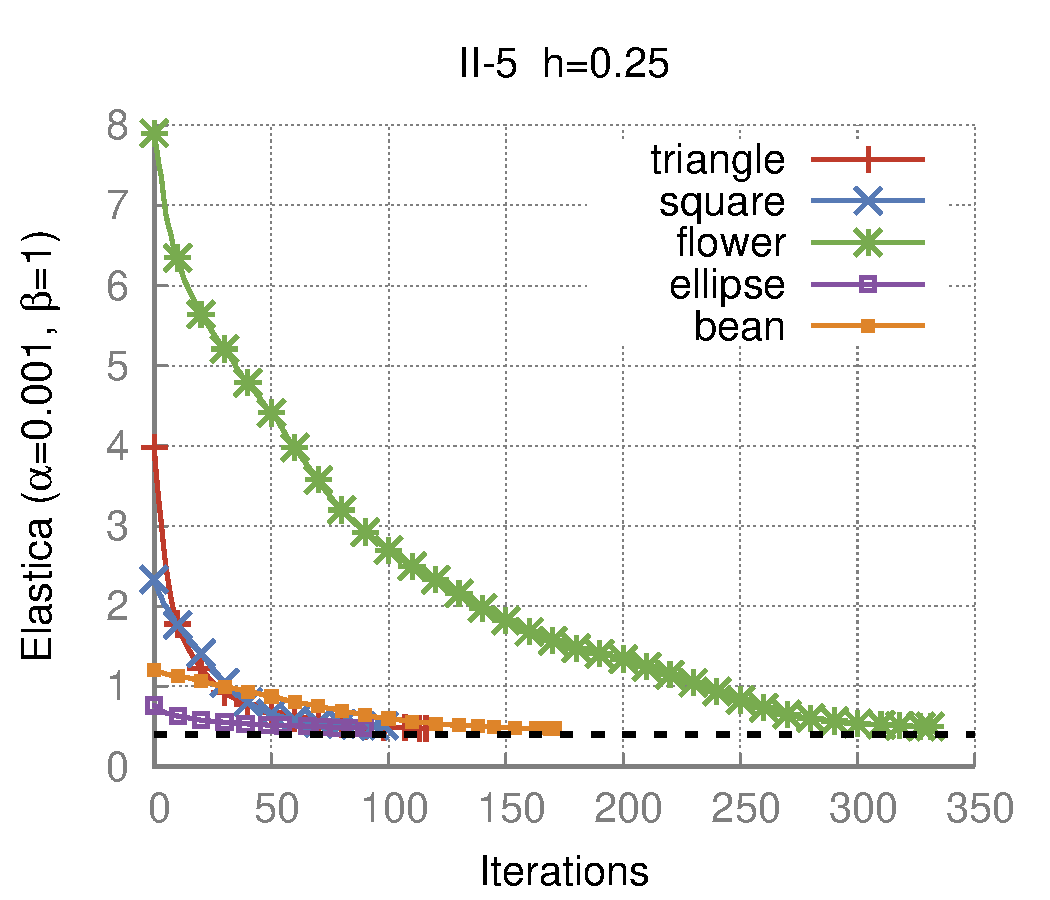
\includegraphics[scale=0.4]{figures/chapter5/flow/plots/summary/lp_0.001/summary-ii5.pdf}
}%
\caption{\daniel{\textbf{Free elastica evolution plots for ($\mathbf{\alpha=0.001, \beta=1}$).}} Minimum value attained for the digial elastica in comparison with the global optimum (dashed line) for different curvature estimators and in different scales. The last figure summarizes the digital elastica evolution value for all shapes \daniel{using the II-$5$ estimator and}  grid step $h=0.25$.}
\label{fig:local-comb-estimators-plots-lp0001}
\end{figure}


\begin{figure}[hp!]
	\center
	\begin{tabular}{ccc}
		$h=1.0$ & $h=0.5$ & $h=0.25$ \\[2em]
	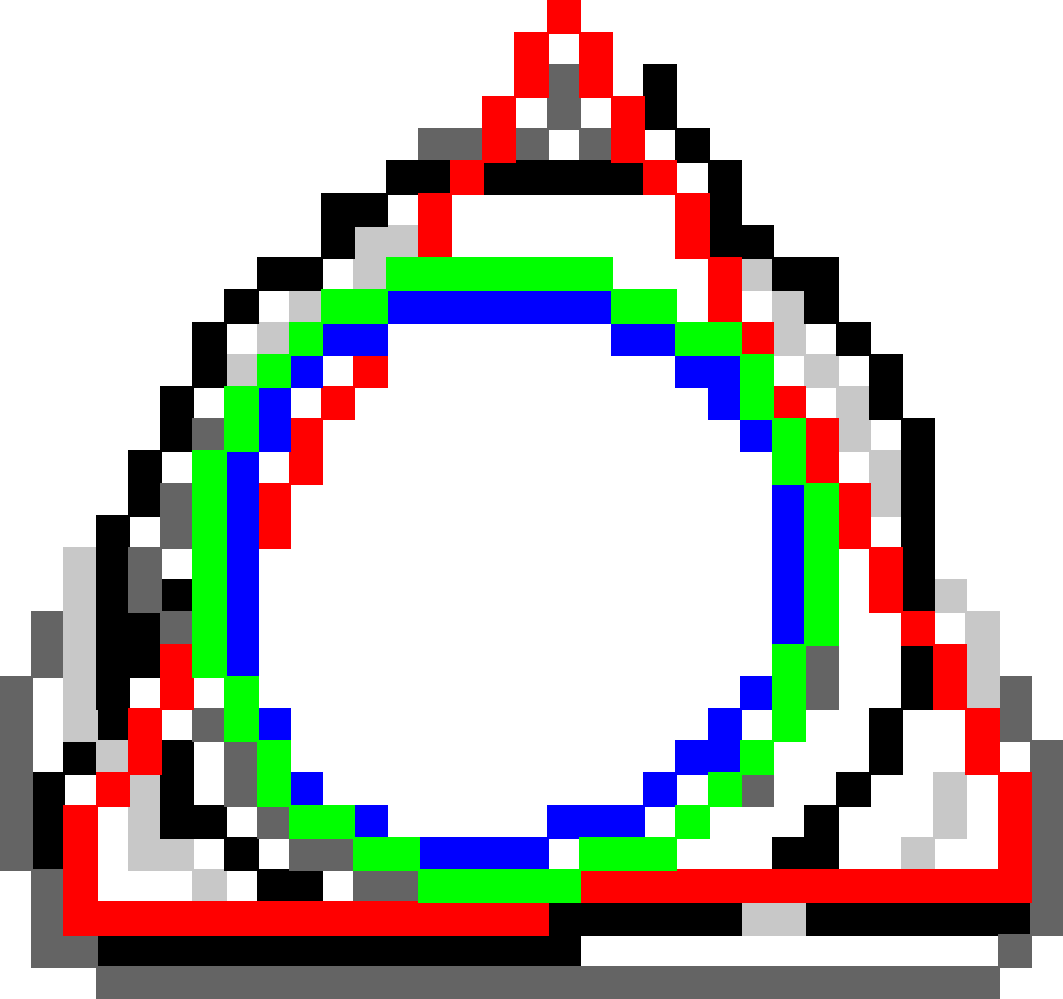
\includegraphics[scale=0.185]{figures/chapter5/flow/triangle/radius_5/ii/elastica/len_pen_0.01000/jonctions_1/curve_segs_4/best/gs_1.00000/summary.pdf} &
	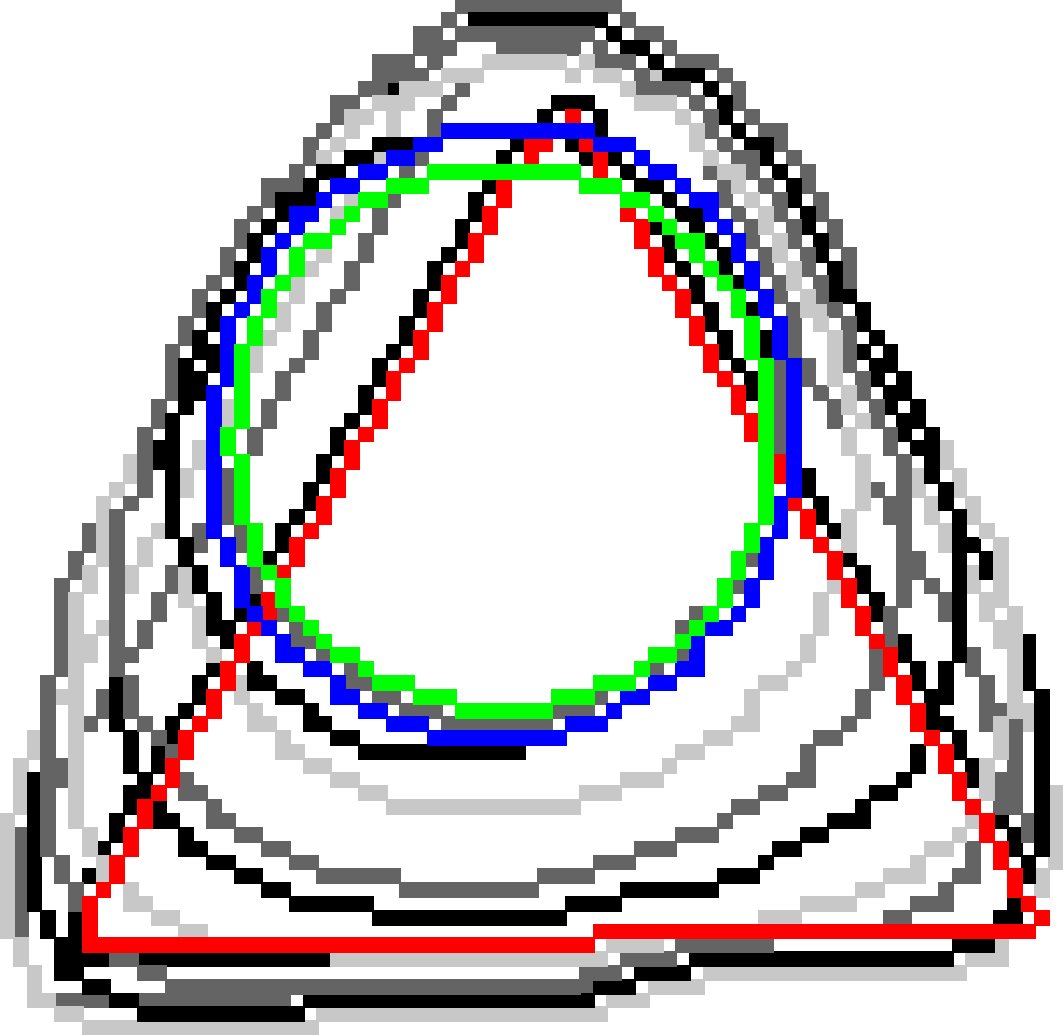
\includegraphics[scale=0.185]{figures/chapter5/flow/triangle/radius_5/ii/elastica/len_pen_0.01000/jonctions_1/curve_segs_4/best/gs_0.50000/summary.pdf} &
	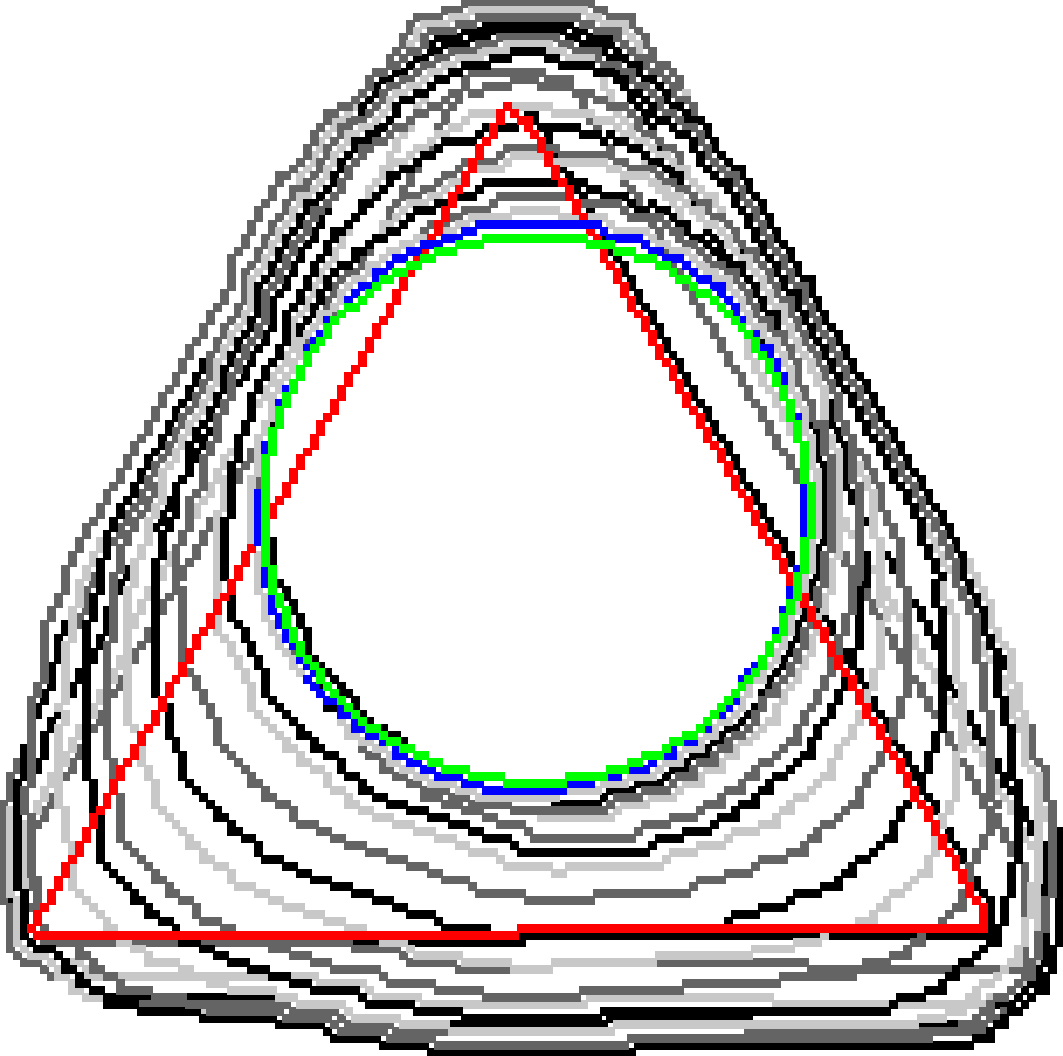
\includegraphics[scale=0.185]{figures/chapter5/flow/triangle/radius_5/ii/elastica/len_pen_0.01000/jonctions_1/curve_segs_4/best/gs_0.25000/summary.pdf}\\[2em]
		
	
\includegraphics[scale=0.17]{figures/chapter5/flow/square/radius_5/ii/elastica/len_pen_0.01000/jonctions_1/curve_segs_4/best/gs_1.00000/summary.pdf} &
	
	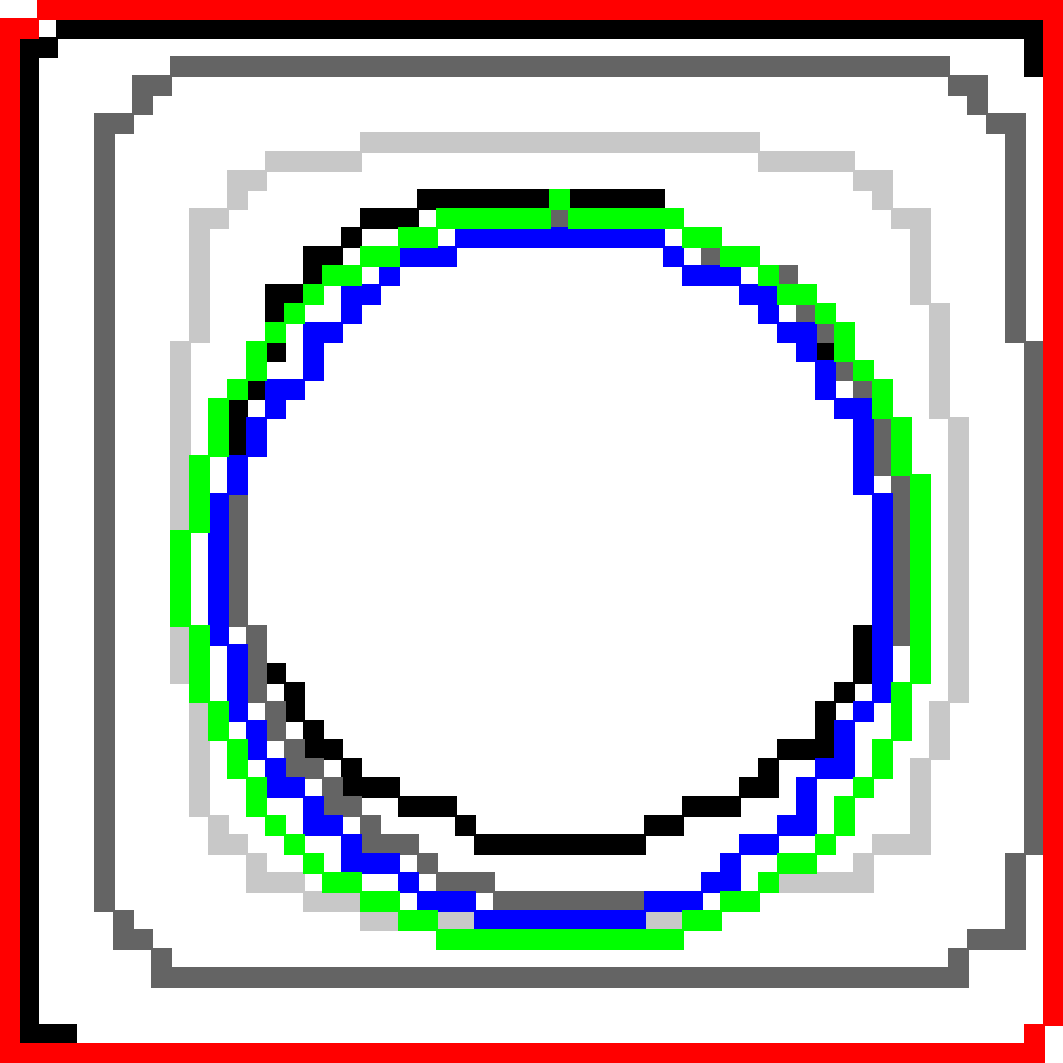
\includegraphics[scale=0.17]{figures/chapter5/flow/square/radius_5/ii/elastica/len_pen_0.01000/jonctions_1/curve_segs_4/best/gs_0.50000/summary.pdf} &	
	
	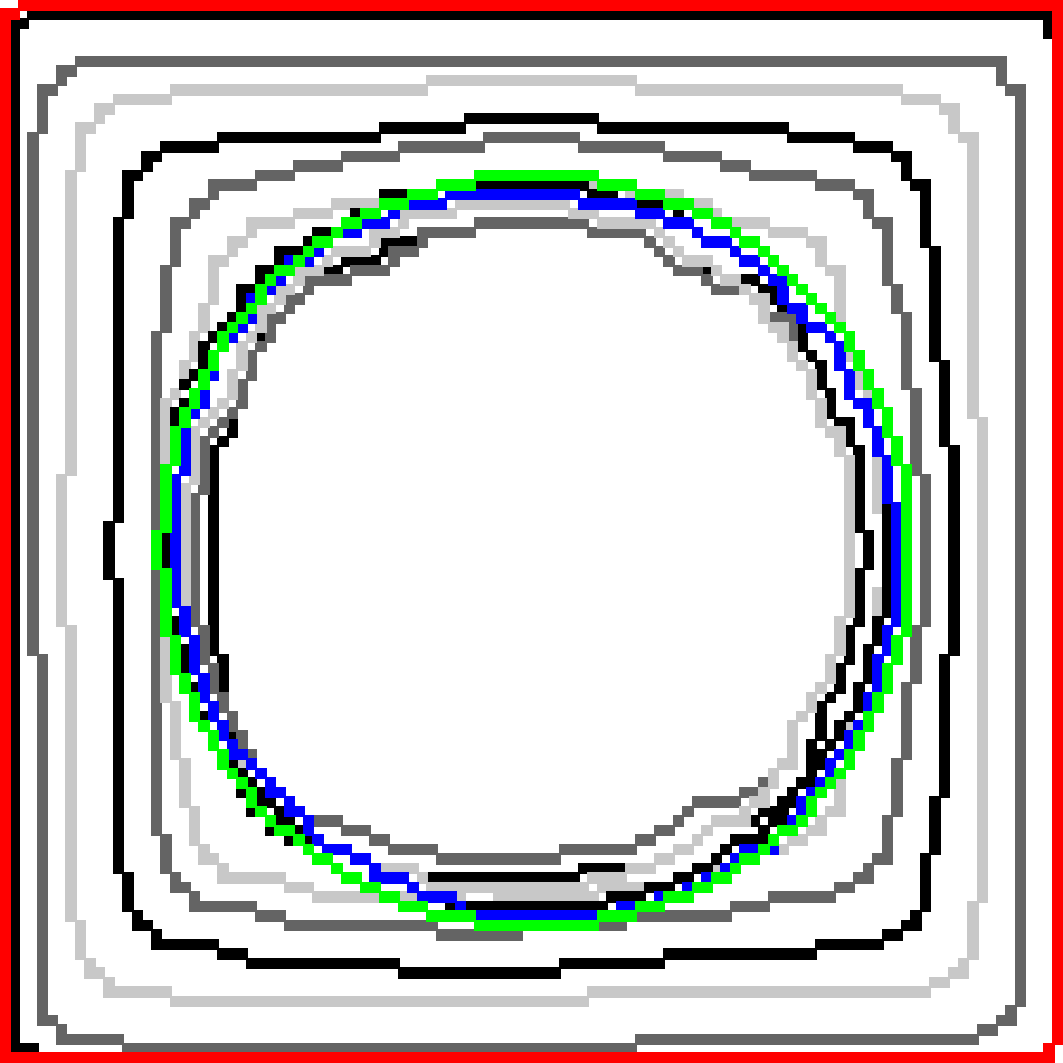
\includegraphics[scale=0.17]{figures/chapter5/flow/square/radius_5/ii/elastica/len_pen_0.01000/jonctions_1/curve_segs_4/best/gs_0.25000/summary.pdf}\\[2em]
	
	
	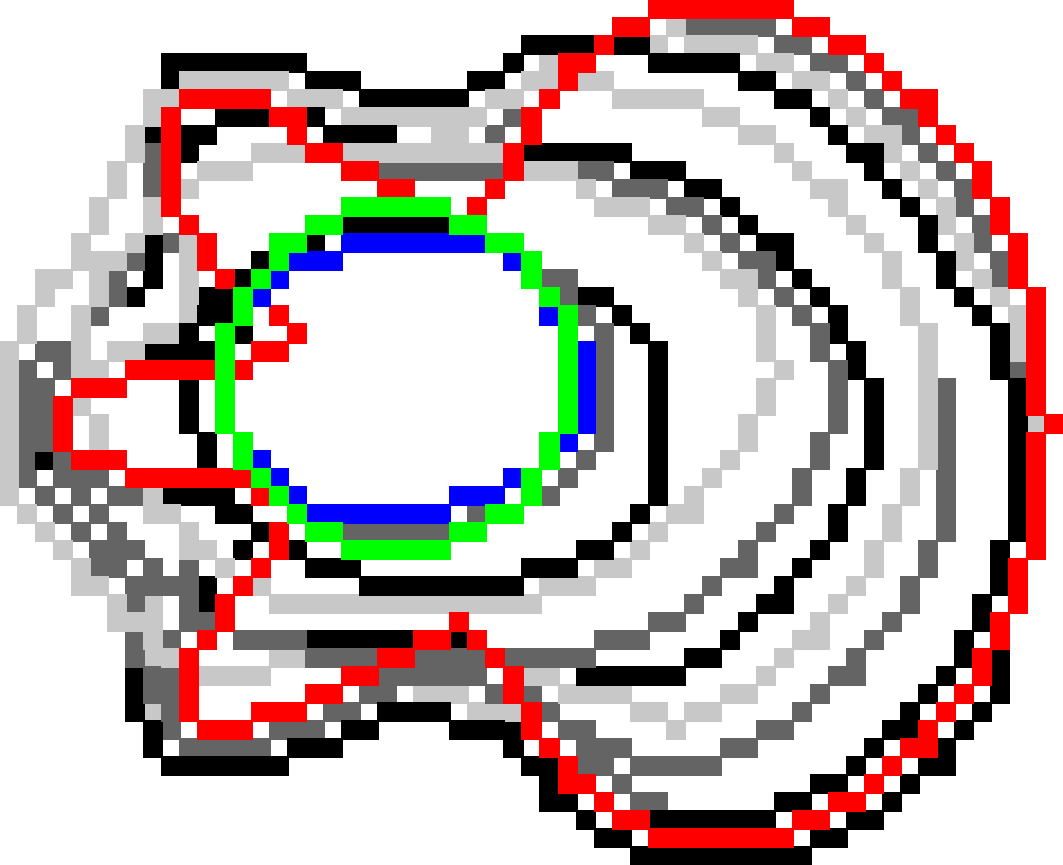
\includegraphics[scale=0.25]{figures/chapter5/flow/flower/radius_5/ii/elastica/len_pen_0.01000/jonctions_1/curve_segs_4/best/gs_1.00000/summary.pdf} &		
	
	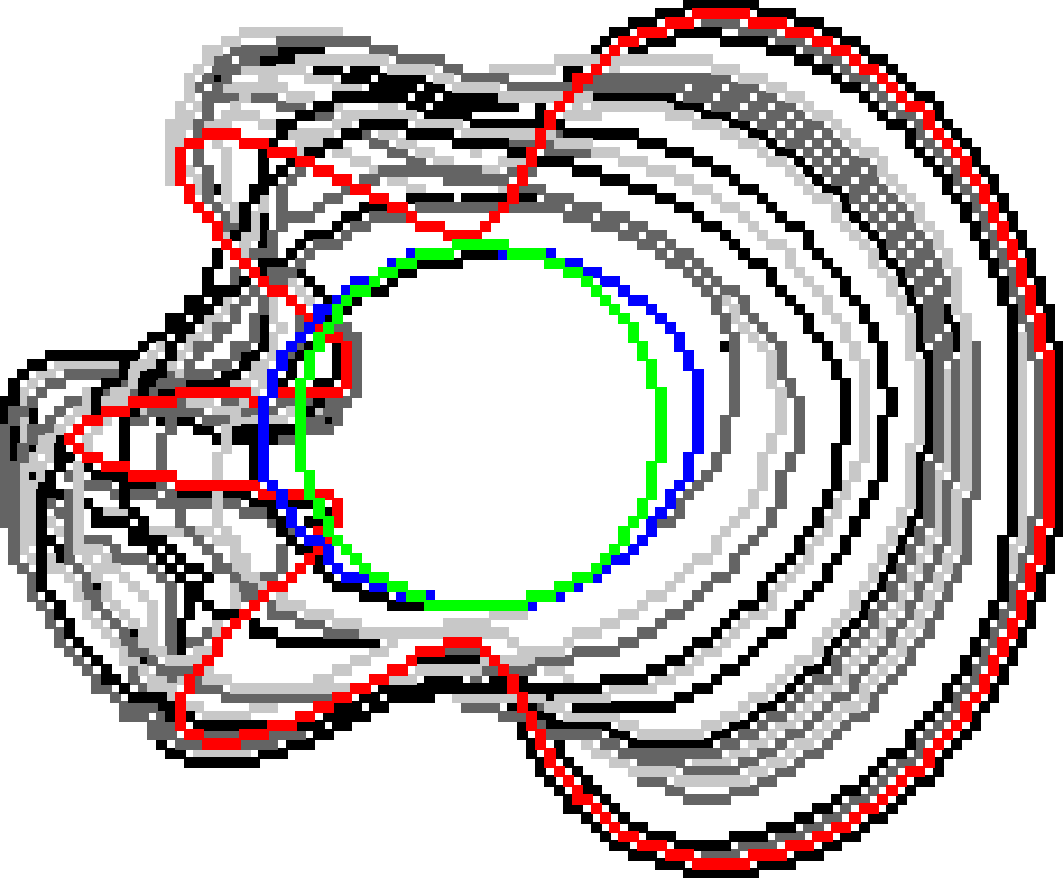
\includegraphics[scale=0.25]{figures/chapter5/flow/flower/radius_5/ii/elastica/len_pen_0.01000/jonctions_1/curve_segs_4/best/gs_0.50000/summary.pdf} &

	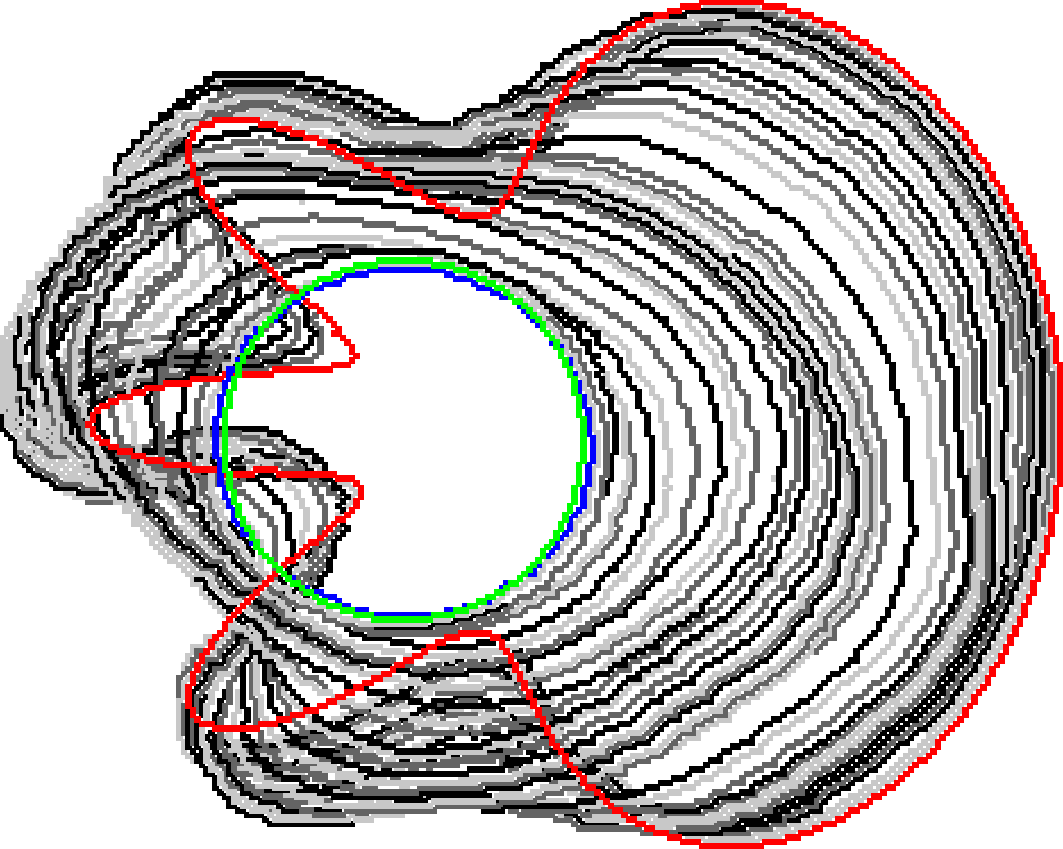
\includegraphics[scale=0.25]{figures/chapter5/flow/flower/radius_5/ii/elastica/len_pen_0.01000/jonctions_1/curve_segs_4/best/gs_0.25000/summary.pdf}\\[2em]	
	
	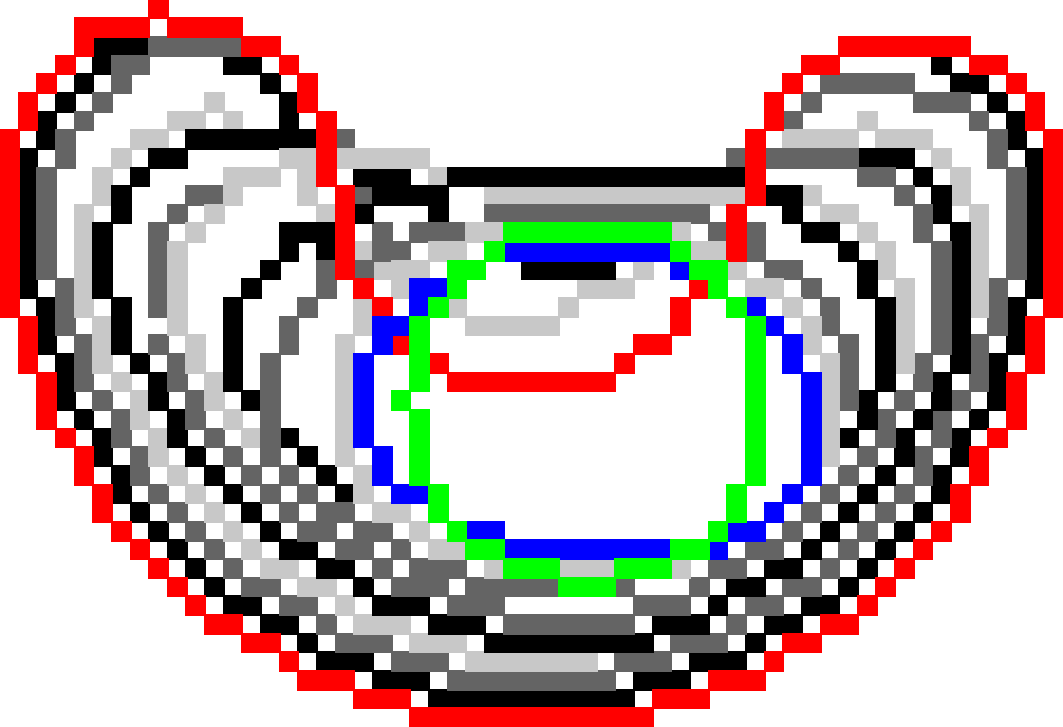
\includegraphics[scale=0.25]{figures/chapter5/flow/bean/radius_5/ii/elastica/len_pen_0.01000/jonctions_1/curve_segs_4/best/gs_1.00000/summary.pdf} &	 
	
	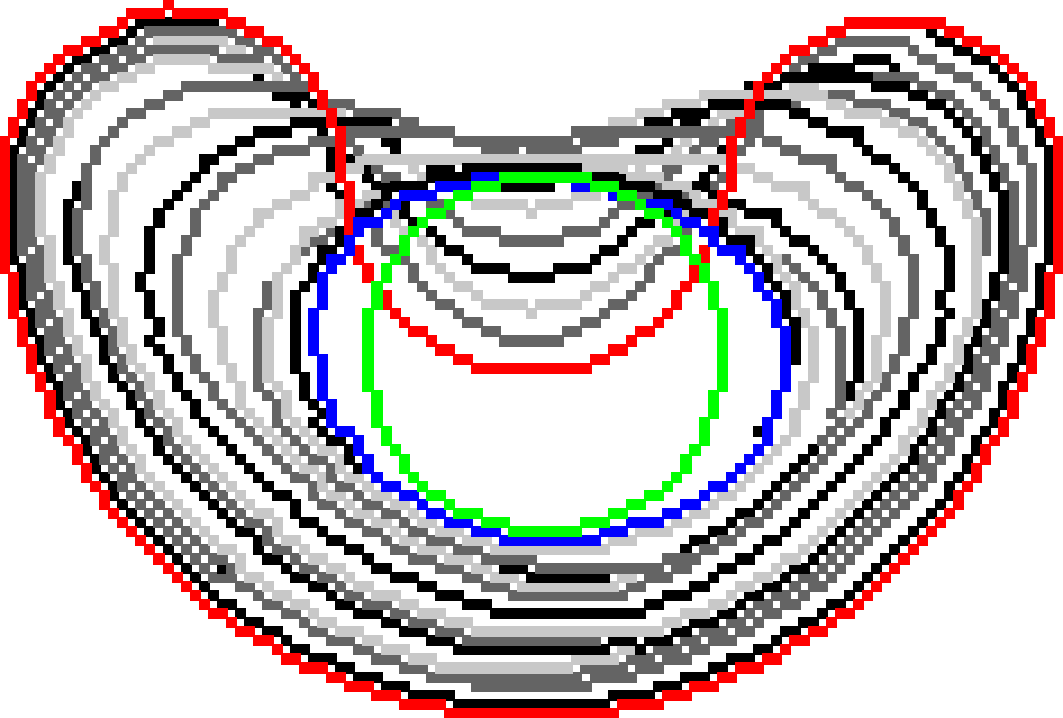
\includegraphics[scale=0.25]{figures/chapter5/flow/bean/radius_5/ii/elastica/len_pen_0.01000/jonctions_1/curve_segs_4/best/gs_0.50000/summary.pdf} &	
	
	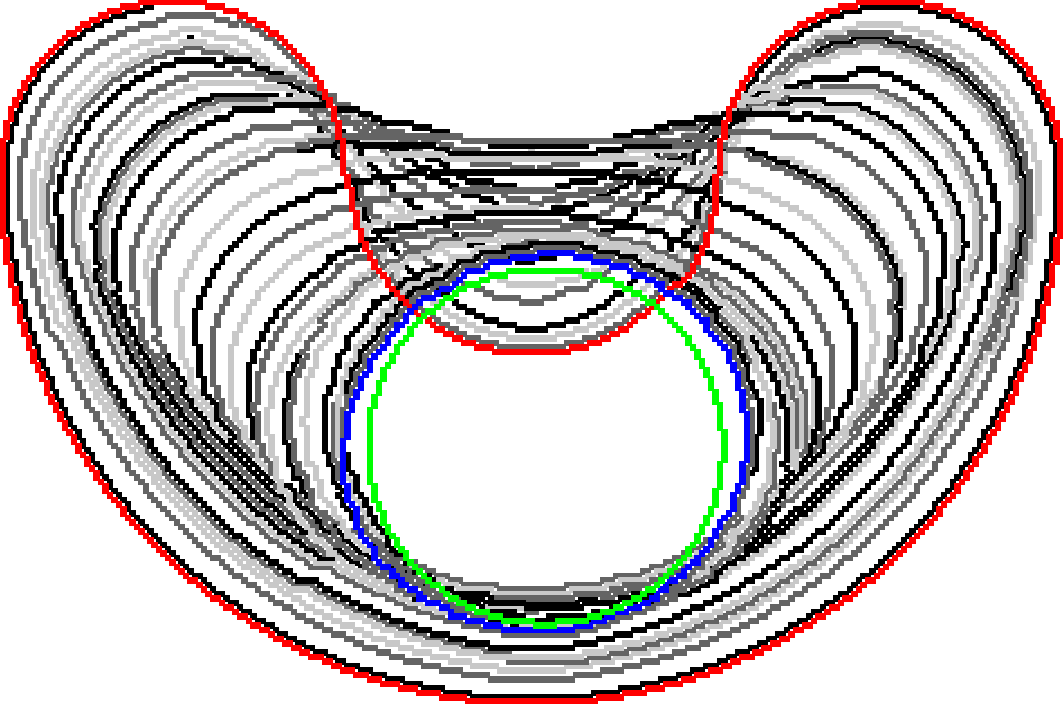
\includegraphics[scale=0.25]{figures/chapter5/flow/bean/radius_5/ii/elastica/len_pen_0.01000/jonctions_1/curve_segs_4/best/gs_0.25000/summary.pdf}\\[2em]			

	
	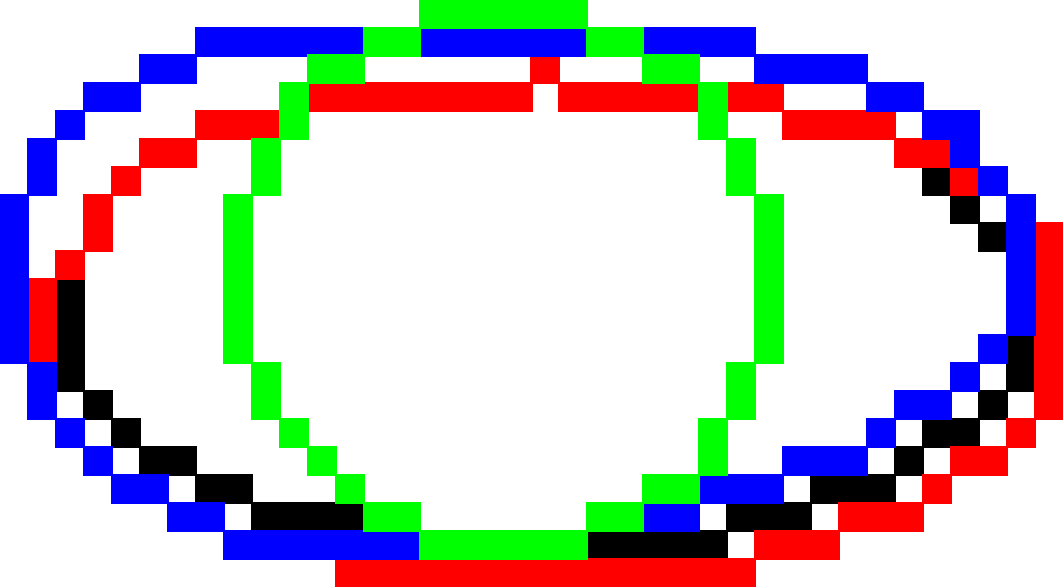
\includegraphics[scale=0.25]{figures/chapter5/flow/ellipse/radius_5/ii/elastica/len_pen_0.01000/jonctions_1/curve_segs_4/best/gs_1.00000/summary.pdf} &

	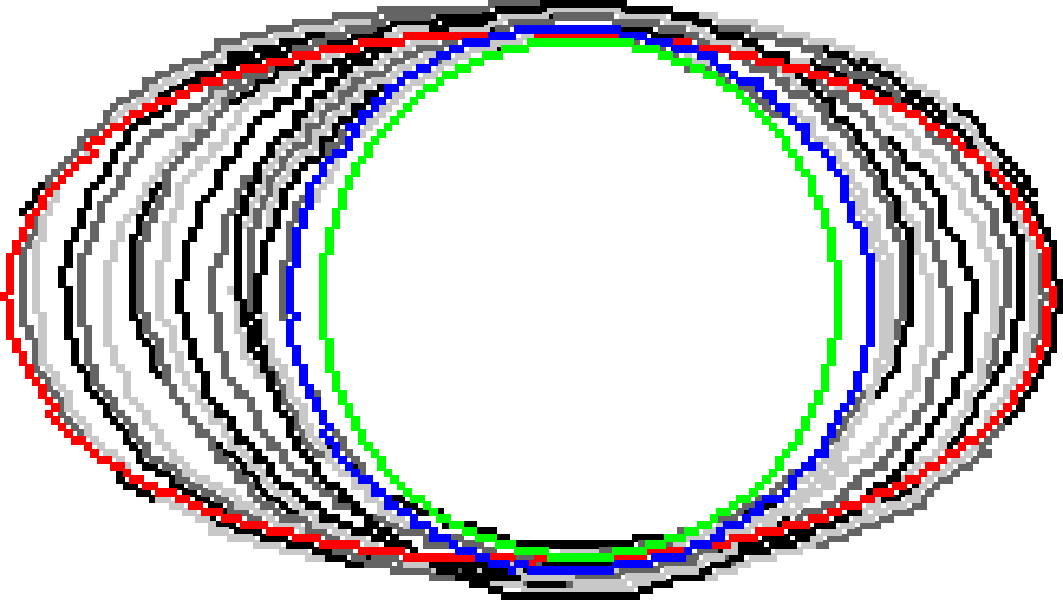
\includegraphics[scale=0.25]{figures/chapter5/flow/ellipse/radius_5/ii/elastica/len_pen_0.01000/jonctions_1/curve_segs_4/best/gs_0.25000/summary.pdf} &

	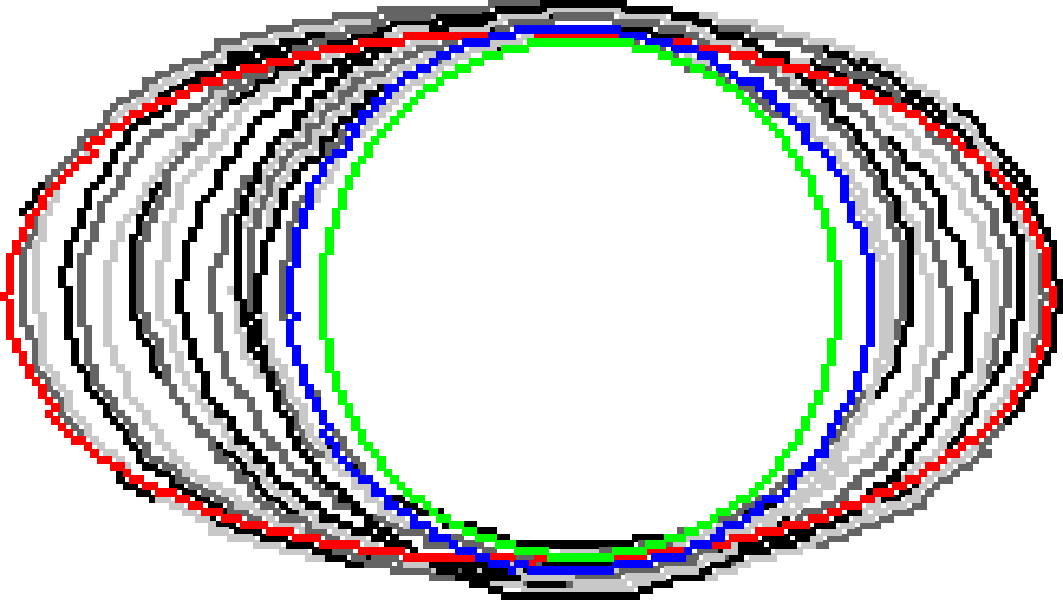
\includegraphics[scale=0.25]{figures/chapter5/flow/ellipse/radius_5/ii/elastica/len_pen_0.01000/jonctions_1/curve_segs_4/best/gs_0.25000/summary.pdf}				
\end{tabular}
		\caption{\daniel{\textbf{Free elastica results for $\mathbf{(\alpha=0.01,\beta=1)}$.}}LocalSearch algorithm evolutions for several shapes. The initial contour is colored in red; the final contour is colored in blue; and the optimal contour is colored in green.}	
		\label{fig:local-comb-ii5-results}
\end{figure}

\begin{figure}
\center
\begin{tabular}{cccc}
& $h=1.0$ & $h=0.5$ & $h=0.25$\\[2em]
\multirow{2}{*}{\rotatebox{90}{$n$-neighborhood}} & 
\figTable{0.25}{figures/chapter5/flow/triangle/radius_3/mdca/elastica/len_pen_0.01000/jonctions_1/curve_segs_4/best/gs_1.00000/summary.pdf} &
\figTable{0.25}{figures/chapter5/flow/triangle/radius_3/mdca/elastica/len_pen_0.01000/jonctions_1/curve_segs_4/best/gs_0.50000/summary.pdf} &
\figTable{0.25}{figures/chapter5/flow/triangle/radius_3/mdca/elastica/len_pen_0.01000/jonctions_1/curve_segs_4/best/gs_0.25000/summary.pdf}\\
& \figTable{0.25}{figures/chapter5/flow/flower/radius_3/mdca/elastica/len_pen_0.01000/jonctions_1/curve_segs_4/best/gs_1.00000/summary.pdf} &
\figTable{0.25}{figures/chapter5/flow/flower/radius_3/mdca/elastica/len_pen_0.01000/jonctions_1/curve_segs_4/best/gs_0.50000/summary.pdf} &
\figTable{0.25}{figures/chapter5/flow/flower/radius_3/mdca/elastica/len_pen_0.01000/jonctions_1/curve_segs_4/best/gs_0.25000/summary.pdf}\\[6em]

\hline\\[1em]

\multirow{2}{*}{\rotatebox{90}{Extended $n$-neighborhood}} & 
\figTable{0.25}{figures/chapter5/mdca-larger-neighborhood/triangle/0.01/1.0/summary.pdf} &
\figTable{0.25}{figures/chapter5/mdca-larger-neighborhood/triangle/0.01/0.5/summary.pdf} &
\figTable{0.25}{figures/chapter5/mdca-larger-neighborhood/triangle/0.01/0.25/summary.pdf}\\

& \figTable{0.25}{figures/chapter5/mdca-larger-neighborhood/flower/0.01/1.0/summary.pdf} &
\figTable{0.25}{figures/chapter5/mdca-larger-neighborhood/flower/0.01/0.5/summary.pdf} &
\figTable{0.25}{figures/chapter5/mdca-larger-neighborhood/flower/0.01/0.25/summary.pdf}


\end{tabular}
\caption{\daniel{\textbf{Effects of an extended neighborhood in the MDCA evolution.}}In the top row, the MDCA evolution for the neighborhood as presented in~\cref{ch5:alg:local-search}. In the bottom row, the flow using the extended neighborhood. The extended neighborhood additionally includes the $n$-neighborhood of the dilation and the erosion of the initial shape by a square of side $1$.}
\label{fig:mdca-larger-neighborhood}
\end{figure}



\begin{figure}[]
\begin{minipage}[b]{0.6\textwidth}
\center
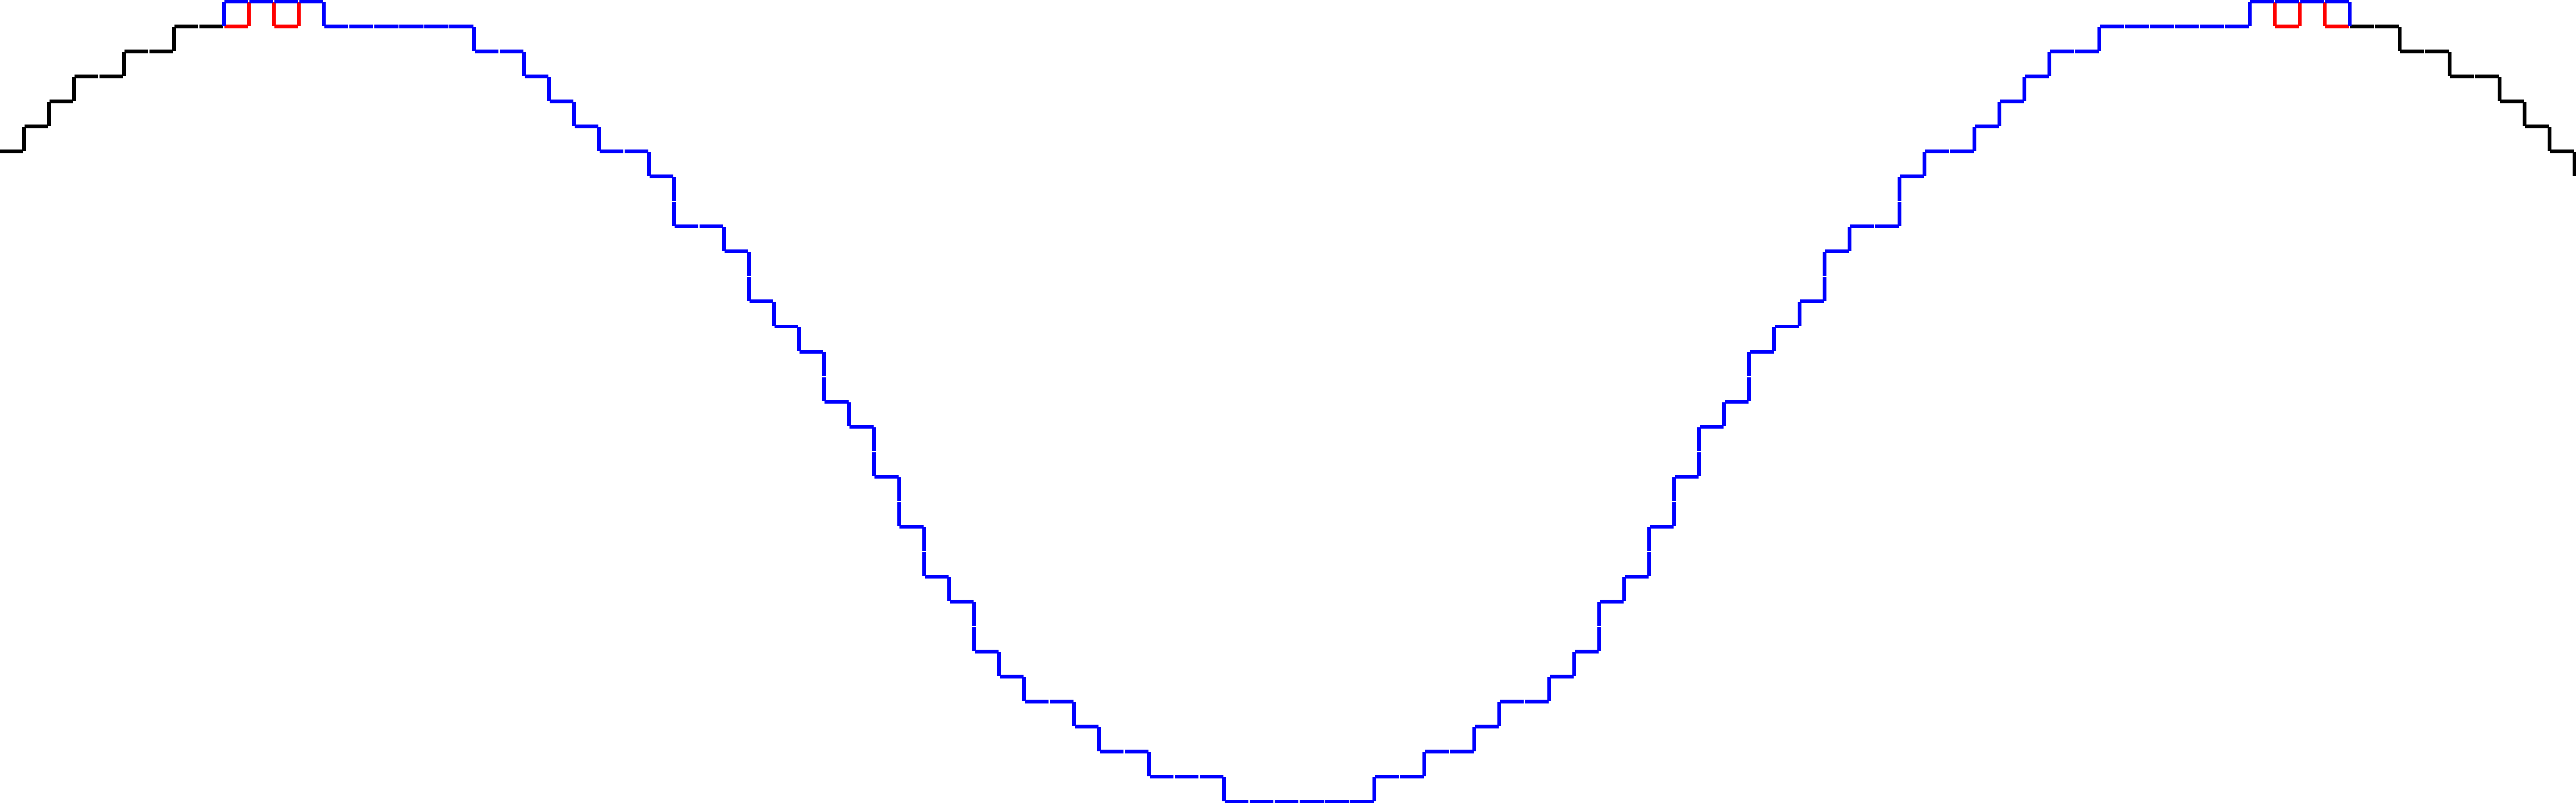
\includegraphics[scale=0.15]{figures/chapter5/mdca-sensitivity/closer-picture.pdf}
\end{minipage}%
\begin{minipage}[b]{0.4\textwidth}
\center
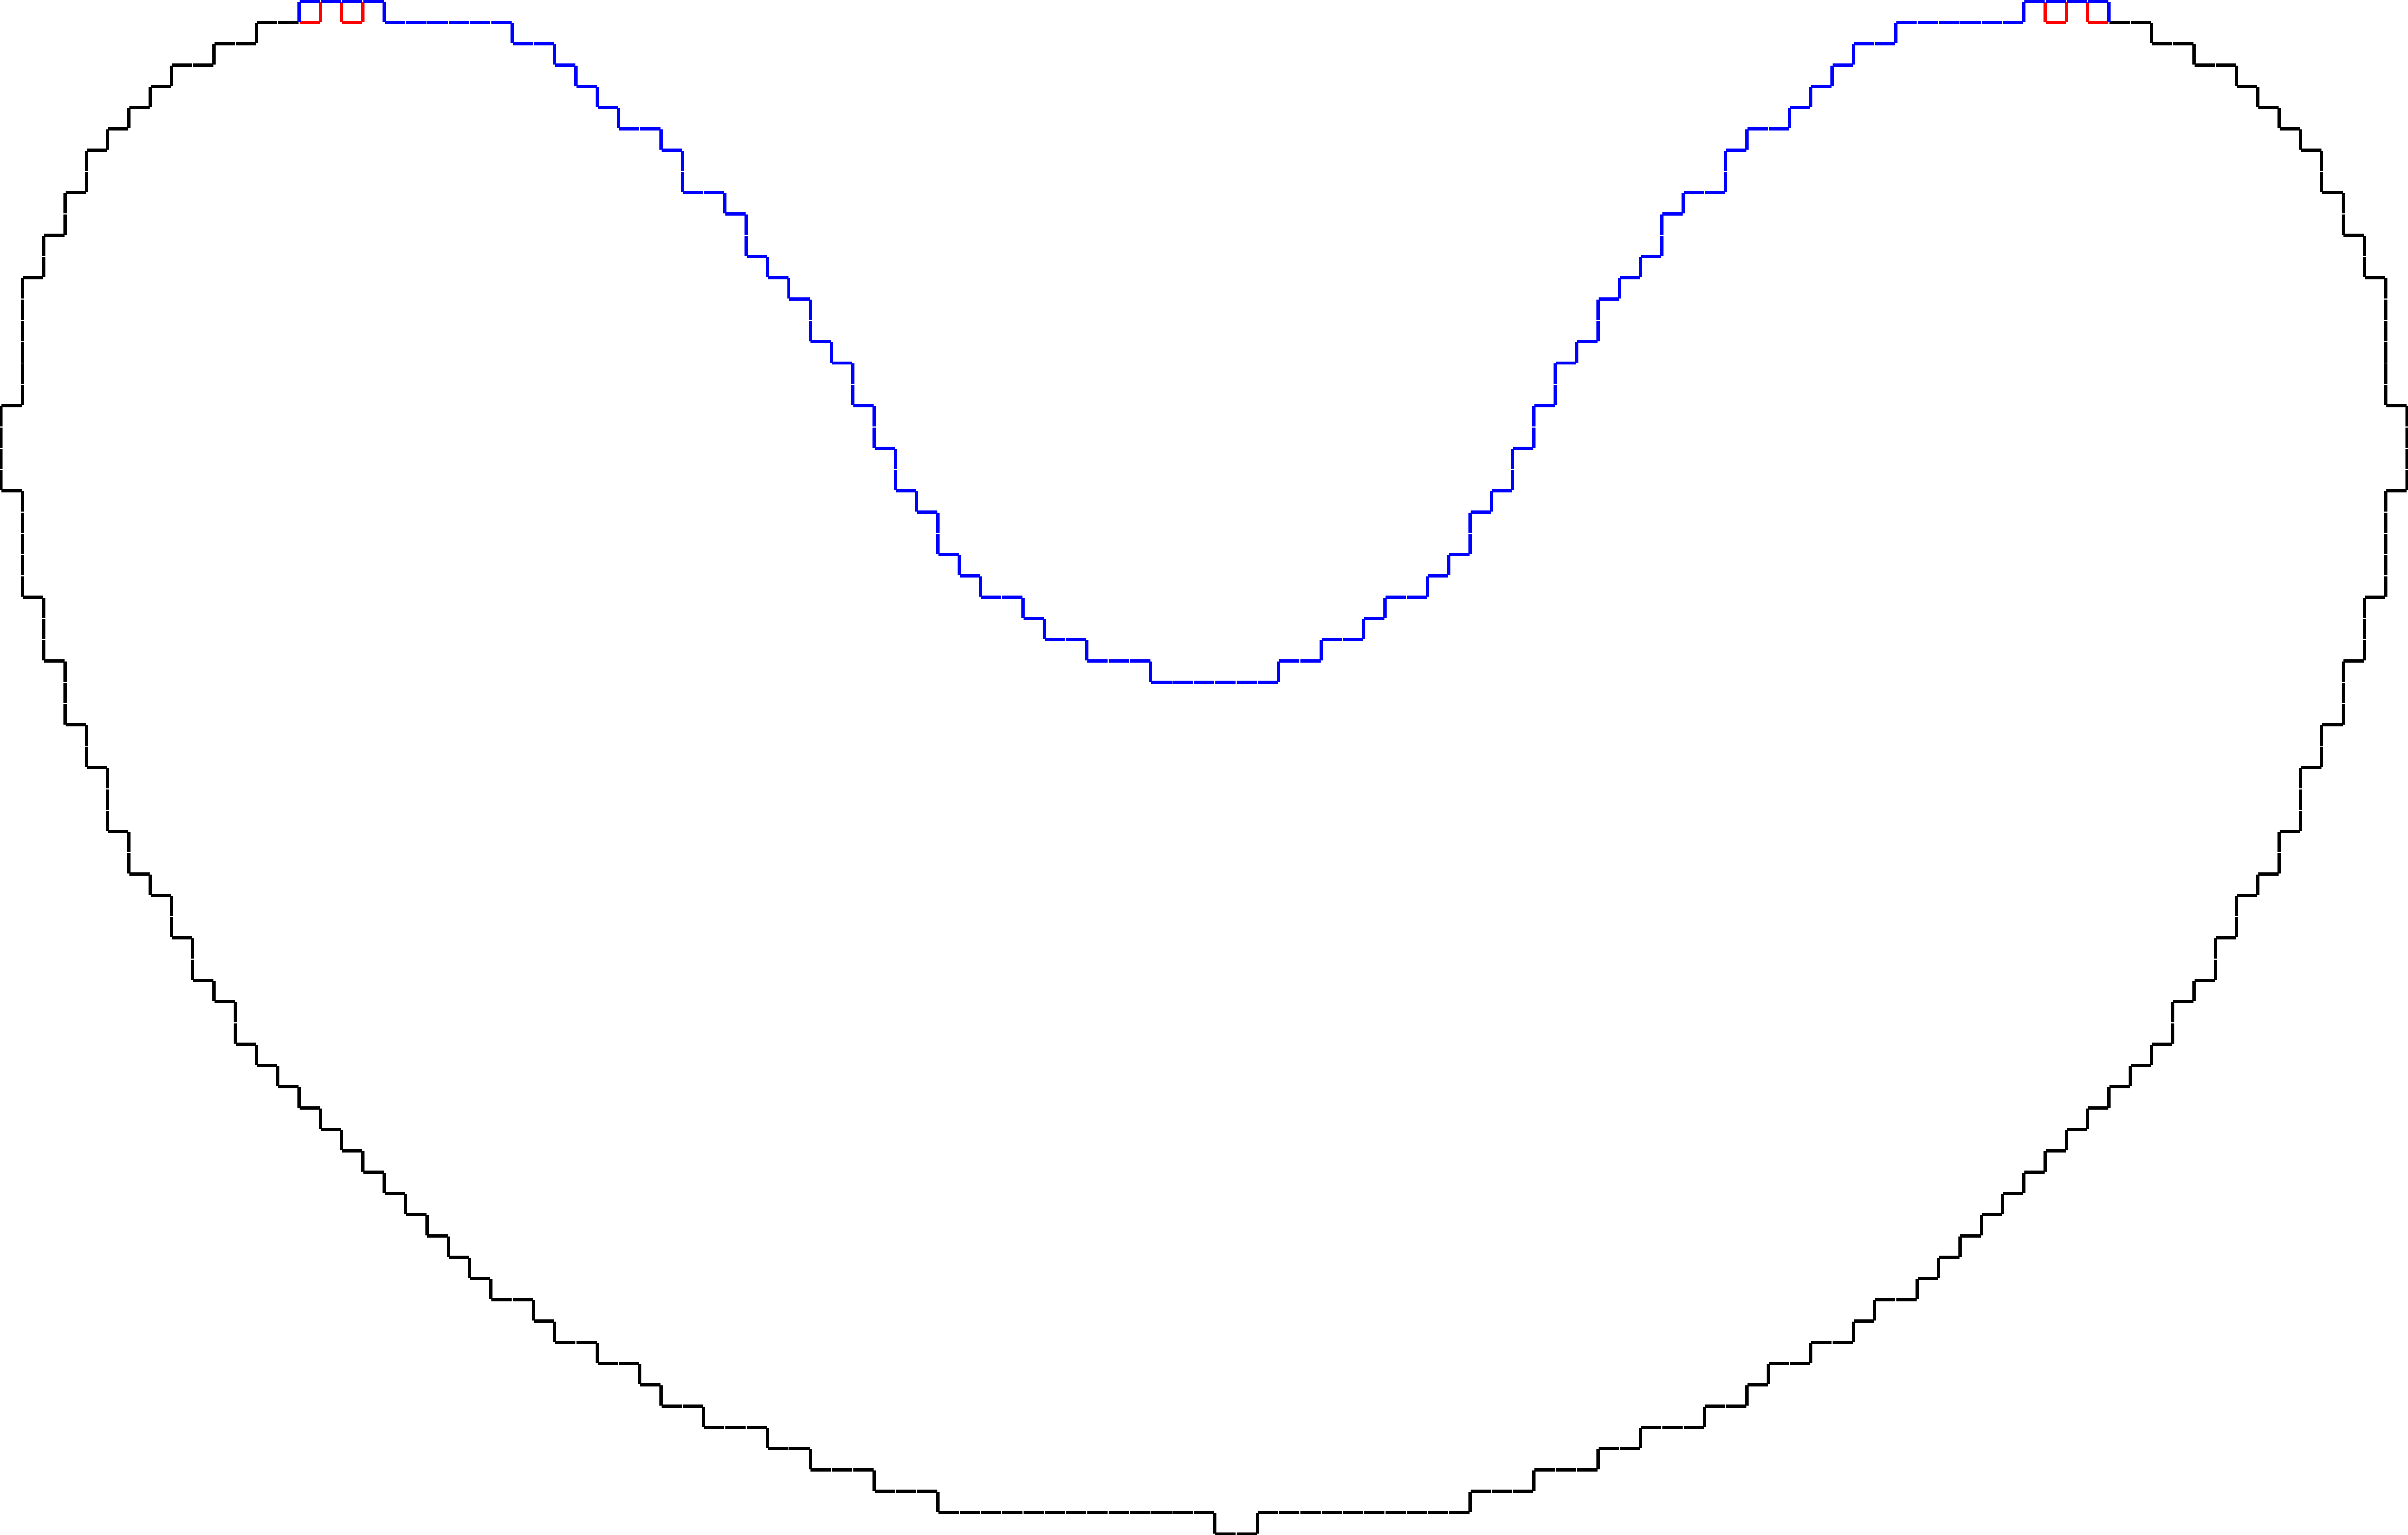
\includegraphics[scale=0.025]{figures/chapter5/mdca-sensitivity/big-picture.pdf}\\\vspace{2em}
\captionsetup{type=table}
\begin{tabular}{r|c|c}
& II-$5$ & MDCA \\
\hline
Red  & 5.54 & 3.93\\
Blue & 5.55 & 3.84\\
\hline
$| \Delta E / \Delta \Ds |$ & 70 & 1400
\end{tabular}
\end{minipage}
\caption{\daniel{\textbf{MDCA sensitivity to noise.}}A slight variation in the shape boundary (in this example, a $0.07\%$ change or $4$ pixels over $5310$) inflicts a considerably higher change in the energy value when using MDCA than when using II. }
\label{fig:mdca-sensitivity}
\end{figure}

\subsection{Constrained elastica}
\label{ch5:subsec:constrained-digital-elastica}

An important advantage of~\cref{ch5:alg:local-search} is that constraints can be imposed with minimum effort. We present results for two types of constraints. In the first type, we force some pixels to be part of the final solution and in the second we impose orientations at the endpoints of a curve, \daniel{as in the general elastica problem}. In~\cref{fig:constrained-elastica} we compare the flows for different values of $\alpha$. 

\daniel{We clearly observe that lower values of $\alpha$ produce longer curves with smoother turns, as expected. However, the local nature of the method may lead to sub-optimal solutions. A global optimization method would not only handle these issues, but would naturally possess the completion property associated with the squared curvature, which may be damped by local approaches.}
%
%We remark that~\cref{alg:local-search} is sensitive to the parameter $\alpha$. For higher values of $\alpha$, the shapes tends to shrink and the curves are closer to a straight line. For lower values of $\alpha$, the shapes tends to grow and the curves make more turns. 
%
\begin{figure}
\center
\begin{tabular}{ccc}
$\alpha=0.1$ & $\alpha=0.01$ & $\alpha=0.001$\\[2em]
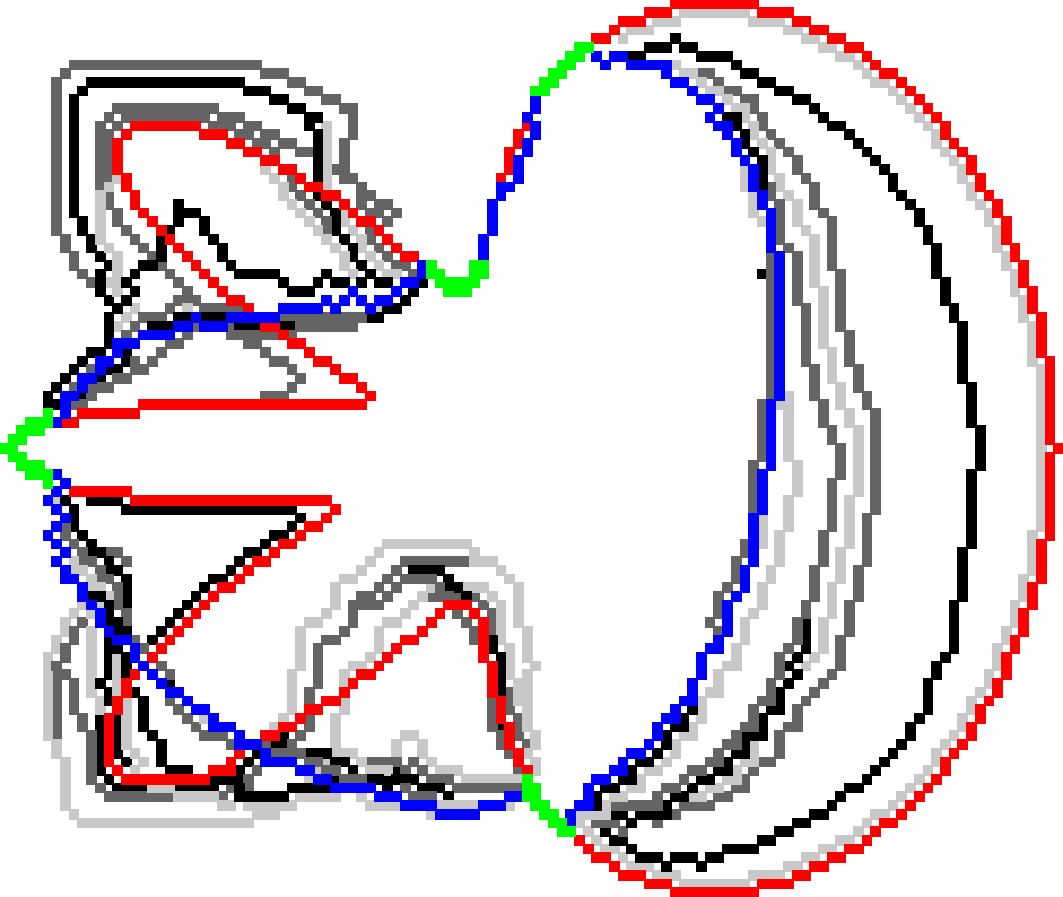
\includegraphics[scale=0.25]{figures/chapter5/fixed-pixels/elastica/len_pen_0.1/flower-1/summary.pdf} &
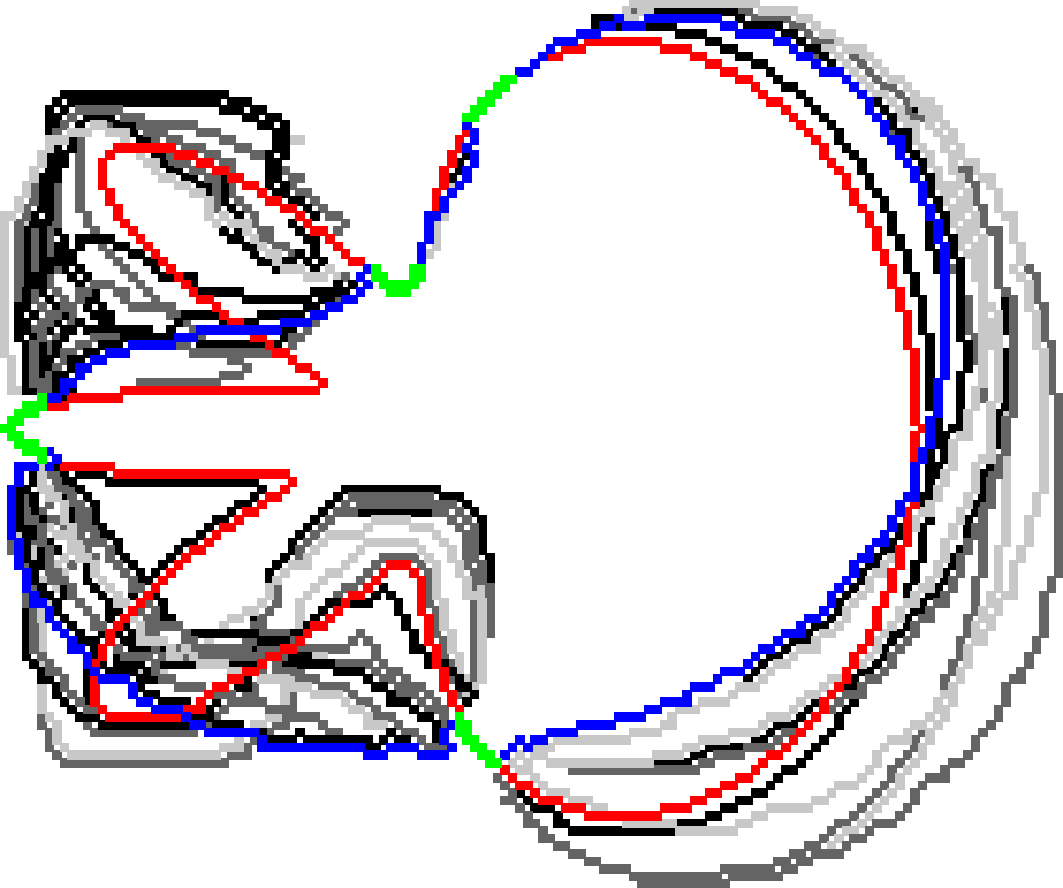
\includegraphics[scale=0.25]{figures/chapter5/fixed-pixels/elastica/len_pen_0.01/flower-1/summary.pdf} &
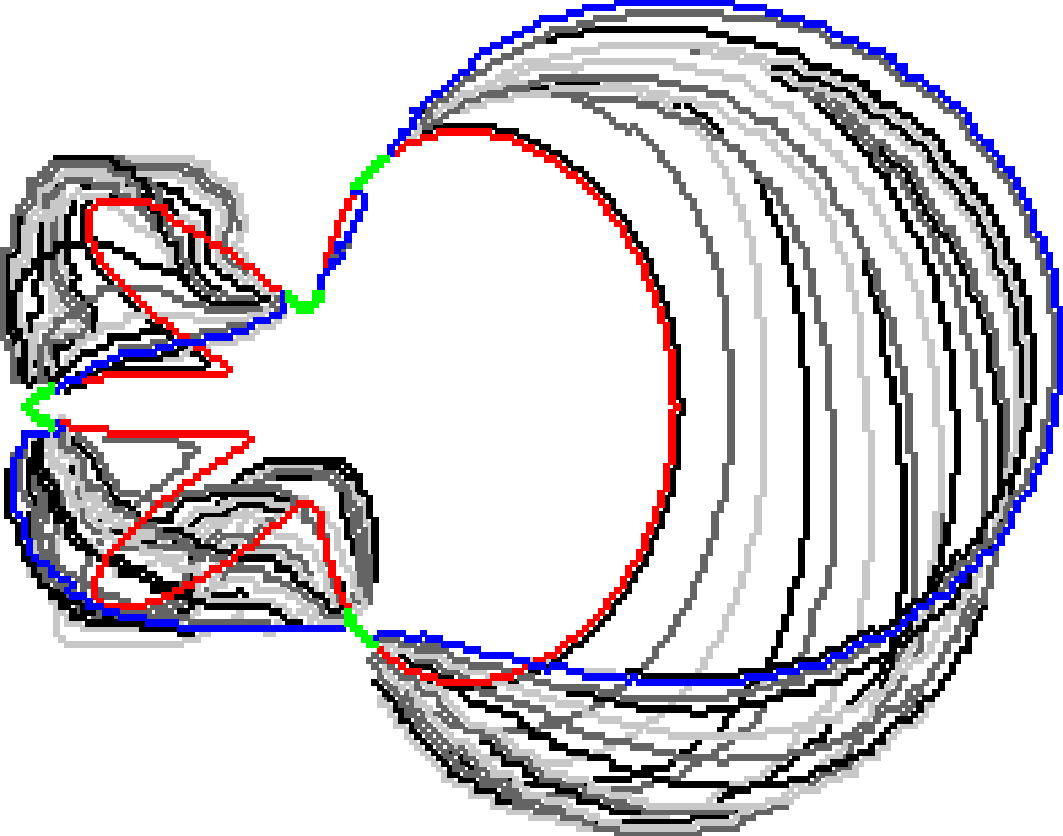
\includegraphics[scale=0.25]{figures/chapter5/fixed-pixels/elastica/len_pen_0.001/flower-1/summary.pdf}\\[2em]
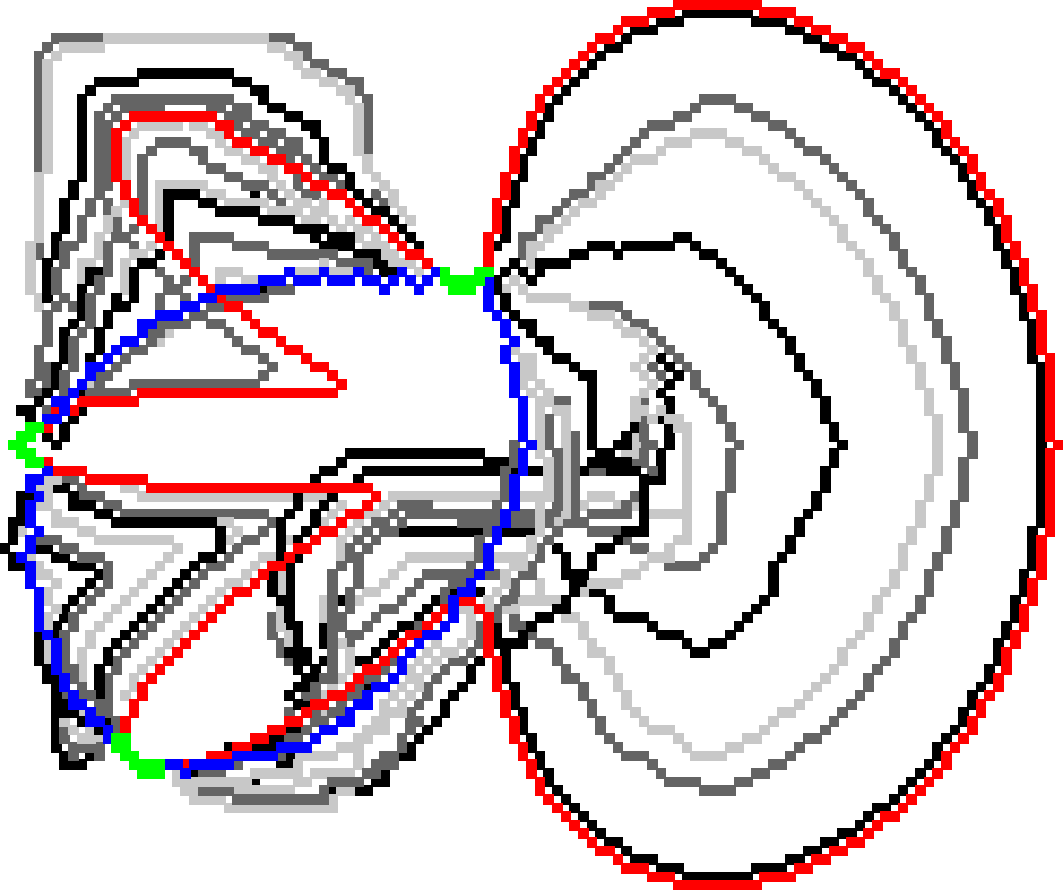
\includegraphics[scale=0.25]{figures/chapter5/fixed-pixels/elastica/len_pen_0.1/flower-2/summary.pdf} &
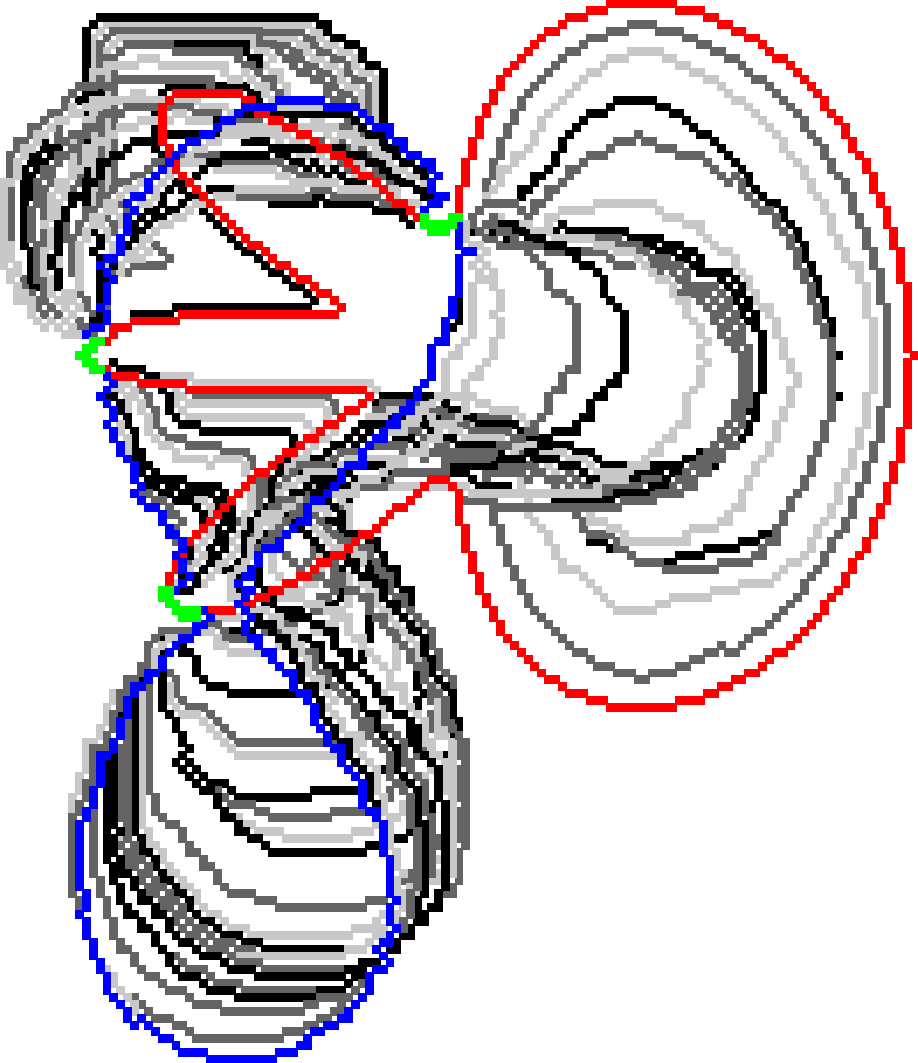
\includegraphics[scale=0.25]{figures/chapter5/fixed-pixels/elastica/len_pen_0.01/flower-2/summary.pdf} &
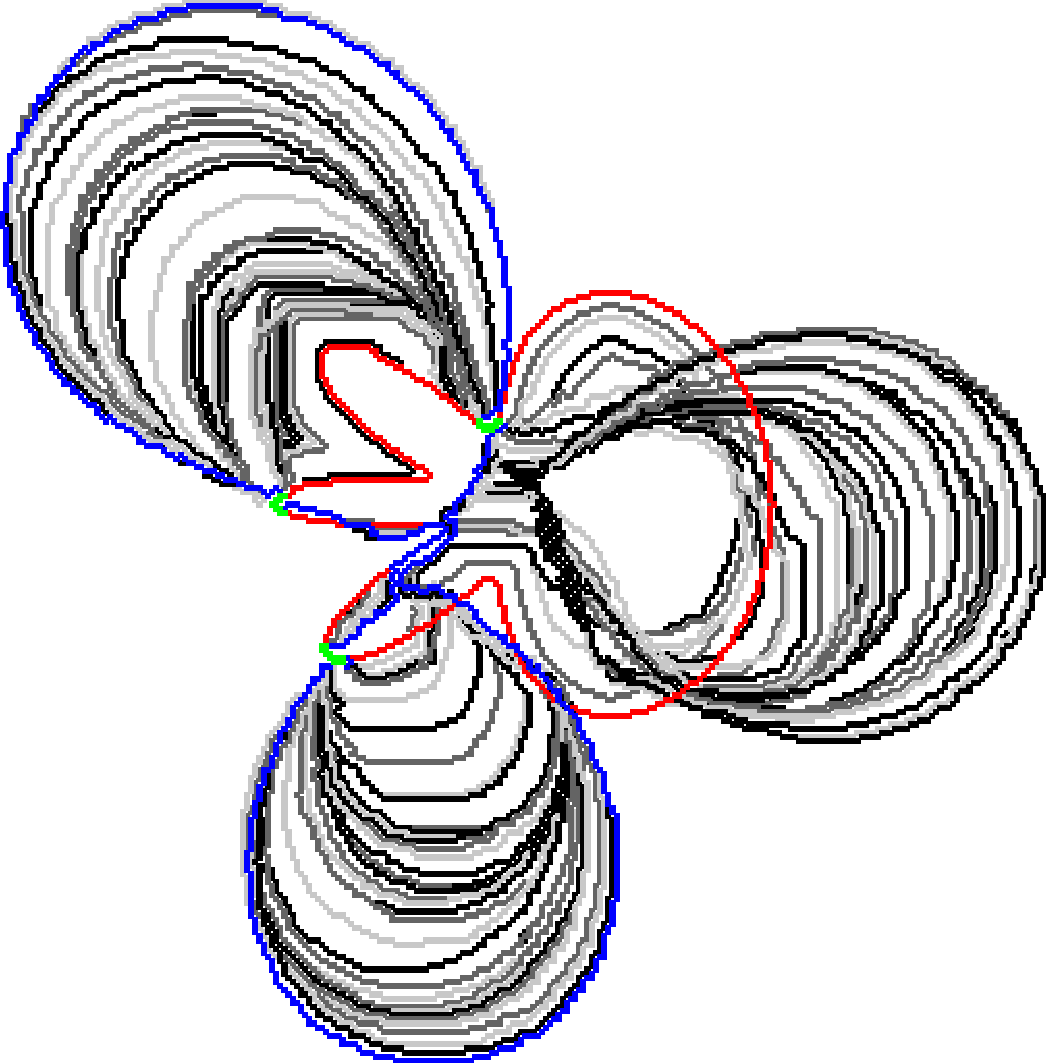
\includegraphics[scale=0.25]{figures/chapter5/fixed-pixels/elastica/len_pen_0.001/flower-2/summary.pdf}\\[2em]
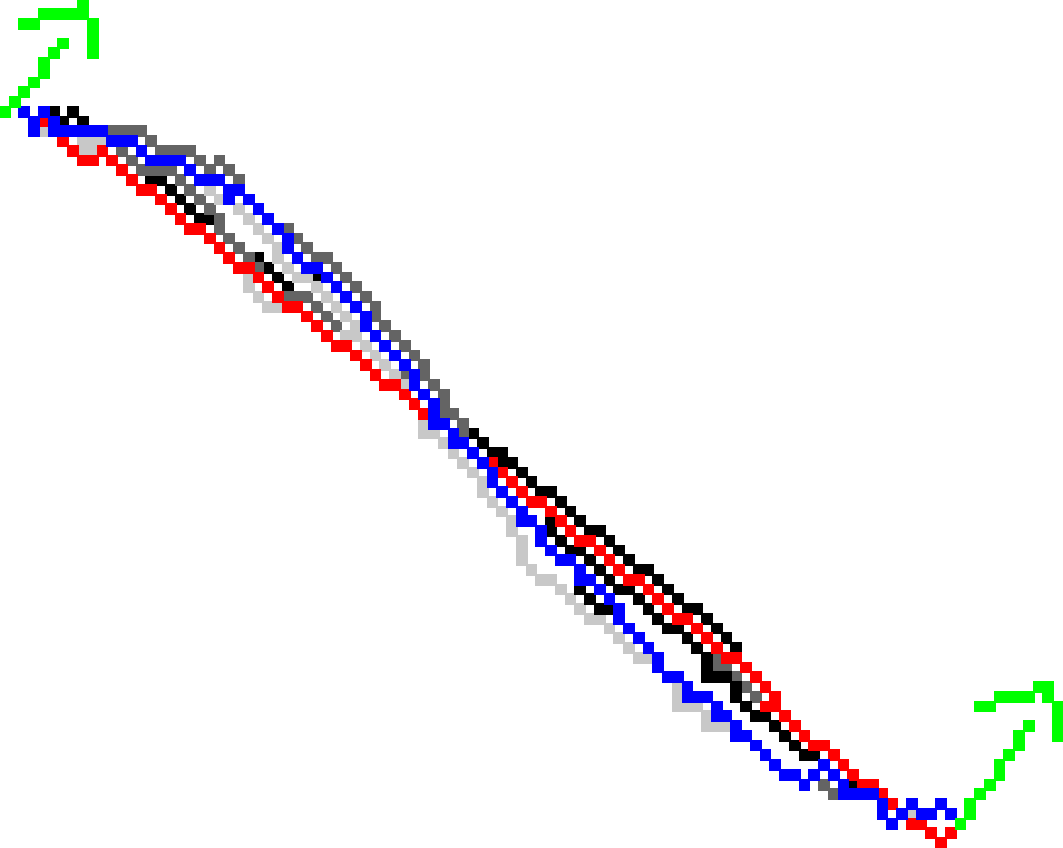
\includegraphics[scale=0.25]{figures/chapter5/fixed-orientations/elastica/len_pen_0.1/curve-2/summary.pdf} &
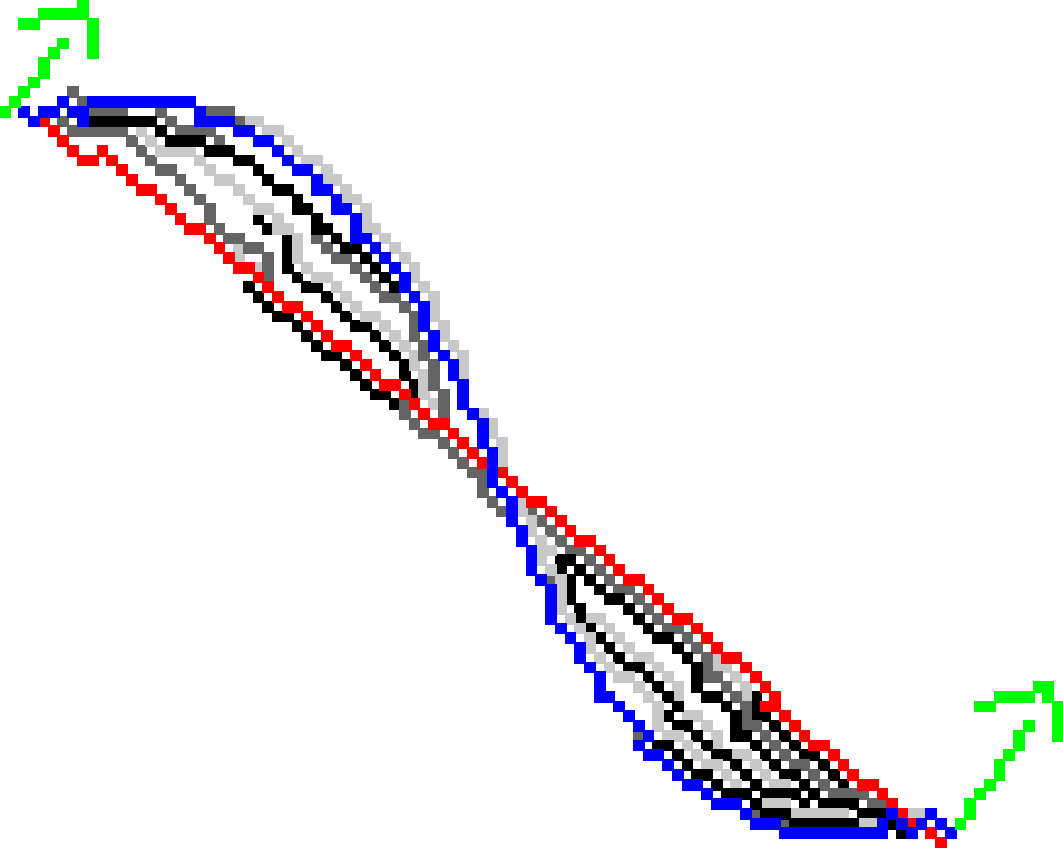
\includegraphics[scale=0.25]{figures/chapter5/fixed-orientations/elastica/len_pen_0.01/curve-2/summary.pdf} &
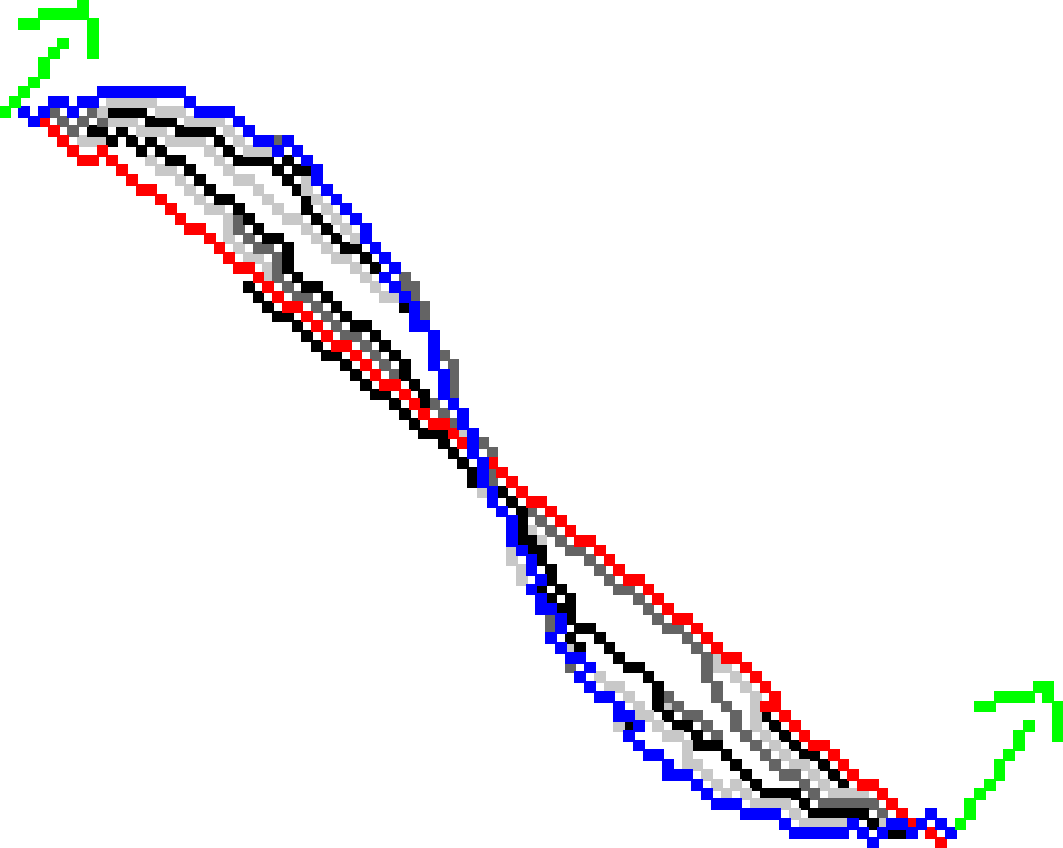
\includegraphics[scale=0.25]{figures/chapter5/fixed-orientations/elastica/len_pen_0.001/curve-2/summary.pdf}\\[2em]
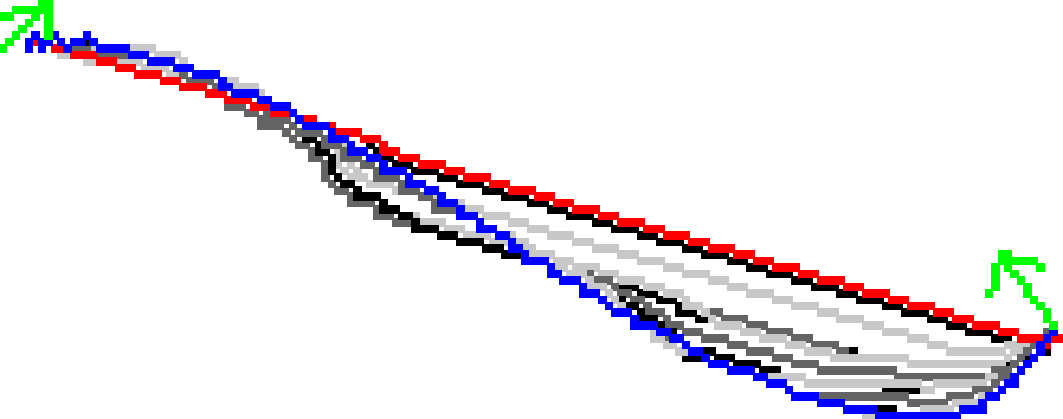
\includegraphics[scale=0.25]{figures/chapter5/fixed-orientations/elastica/len_pen_0.1/curve-3/summary.pdf} &
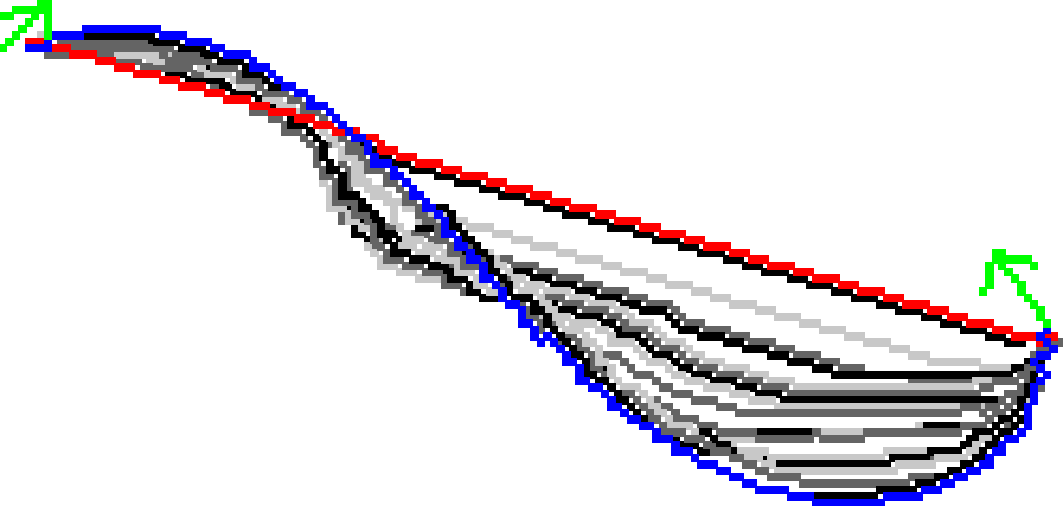
\includegraphics[scale=0.25]{figures/chapter5/fixed-orientations/elastica/len_pen_0.01/curve-3/summary.pdf} &
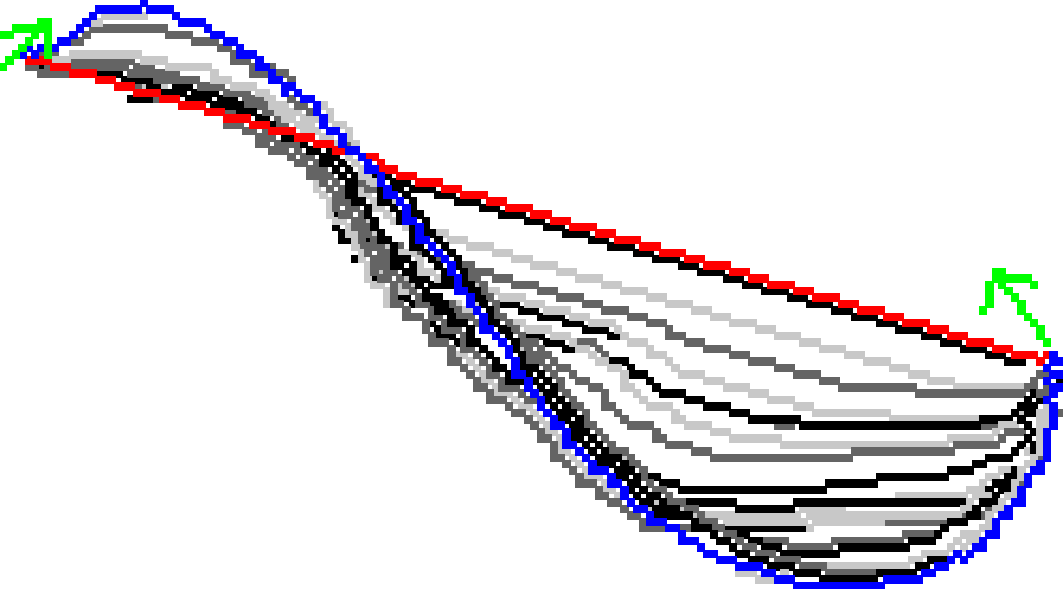
\includegraphics[scale=0.25]{figures/chapter5/fixed-orientations/elastica/len_pen_0.001/curve-3/summary.pdf}
\end{tabular}
\caption{\daniel{\textbf{Constrained elastica results.}} In the first and second rows, the flow obtained by forcing the green pixels to be part of the final solution; In the last two rows, the flow obtained by forcing the orientation at the endpoints of the curves.}
\label{fig:constrained-elastica}

\end{figure}

\subsection{Running time}
\label{ch5:subsec:running-time}

The running time of~\cref{ch5:alg:local-search} is summarized in table~\cref{tab:summary-local-comb-rtime}. All the experiments in this thesis were executed on a $32$-core $2.4Ghz$ CPU. Although its use in practical applications is
limited, we demonstrated that digital estimators are effective in their measurements and the flows evolve as expected, reaching the global optimum for some shapes \daniel{in the free elastica problem}. We
observe that it is a complete digital approach, and we do not suffer from discretization and rounding problems, a common
issue in continuous models.  Furthermore we have checked that this approach works indifferently with Integral Invariant
curvature estimator and Maximal Digital Circular Arc curvature estimator, given an appropriate neighborhood. So the convergence of the digital curvature
estimator seems to be the cornerstone to get a digital curve behaving like a continuous elastica. 

\begin{figure}[h!]
\center
\captionsetup{type=table}
\footnotesize
\begin{tabular}{|l|c|c|c|c|c|c|}
\hline
& \multicolumn{2}{c|}{$h=1.0$} & \multicolumn{2}{c|}{$h=0.5$} & \multicolumn{2}{c|}{$h=0.25$}\\
\hline
& Pixels & Time & Pixels & Time & Pixels & Time\\
\hline
Triangle & 521 & 2s (0.07s/it)  & 2080 & 43s (0.81s/it) & 8315 & 532s(4.8s/it)\\
Square & 841 & 0.9s (0.09s/it) & 3249 & 8s (0.3s/it) & 12769 & 102s (2s/it)\\
Flower & 1641 & 13s (0.24s/it) & 6577 & 209s (1.68s/it) & 26321 & 3534s (12.3s/it)\\
Bean  & 1574 & 7s (0.16s/it) & 6278 & 88s (1.08s/it) & 25130 & 1131s (6.4s/it)\\
Ellipse  & 626 & 1s (0.14s/it) & 2506 & 16s (0.44s/it) & 10038 & 286s (3.1s/it)\\
\hline
\end{tabular}
\caption{\daniel{\textbf{Running time of LocalSearch.}} The running times for the free elastica problem are displayed. \daniel{Notice that even having a similar number of pixels, the square (bean) shape evolves much faster than the triangle (flower).}}
\label{tab:summary-local-comb-rtime} 
\end{figure}





\section{Global optimization}
\label{ch5:sec:global-optimization}
\daniel{As observed in previous section, a global optimization method is important to recover the completion property of curvature, which is useful in inpainting and segmentation of thin and elongated objects.} In this section we turn to a global optimization approach. However, instead of minimizing~\cref{ch5:digital-elastica} we focus on a simplified version of it in which we do not compute the local length estimator. \daniel{This simplification reduces the order of the energy and will likely lead to a practical model.}

\subsection{Simplified digital elastica}
\label{ch5:subsec:simplified-digital-elastica}

The simplified digital elastica is defined as
	\begin{align}
	\hat{E}_{\Theta}^{simp}( D_h(S) ) = \sum_{\dot{\vec{e}} \in \partial_h S}{ \alpha + \beta \hat{\kappa}_{r}^2(D_h(S),\dot{\vec{e}},h) }.
	\label{eq:simplified-digital-elastica}
	\end{align}
%	
%
We argue that~\cref{eq:simplified-digital-elastica} is a reasonable approximation of~\cref{ch5:digital-elastica}. Indeed, executing~\cref{ch5:alg:local-search} to minimize this simplified digital elastica induces very similar results to those for the digital elastica (see~\cref{fig:simplified-elastica}).


\begin{figure}[]
\center
\begin{tabular}{ccc}
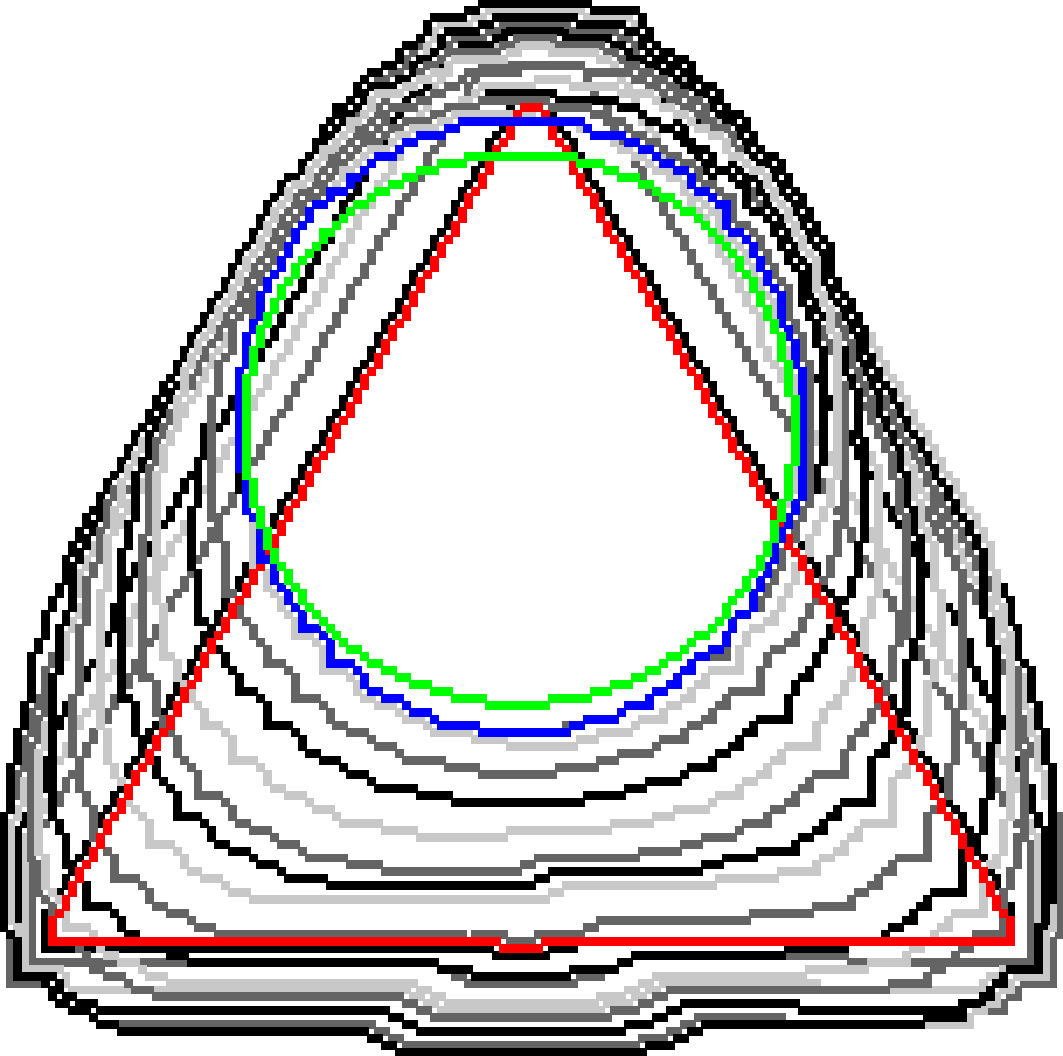
\includegraphics[scale=0.25]{figures/chapter5/flow/triangle/radius_5/ii/selastica/len_pen_0.01000/jonctions_1/curve_segs_4/best/gs_0.25000/summary.pdf} &
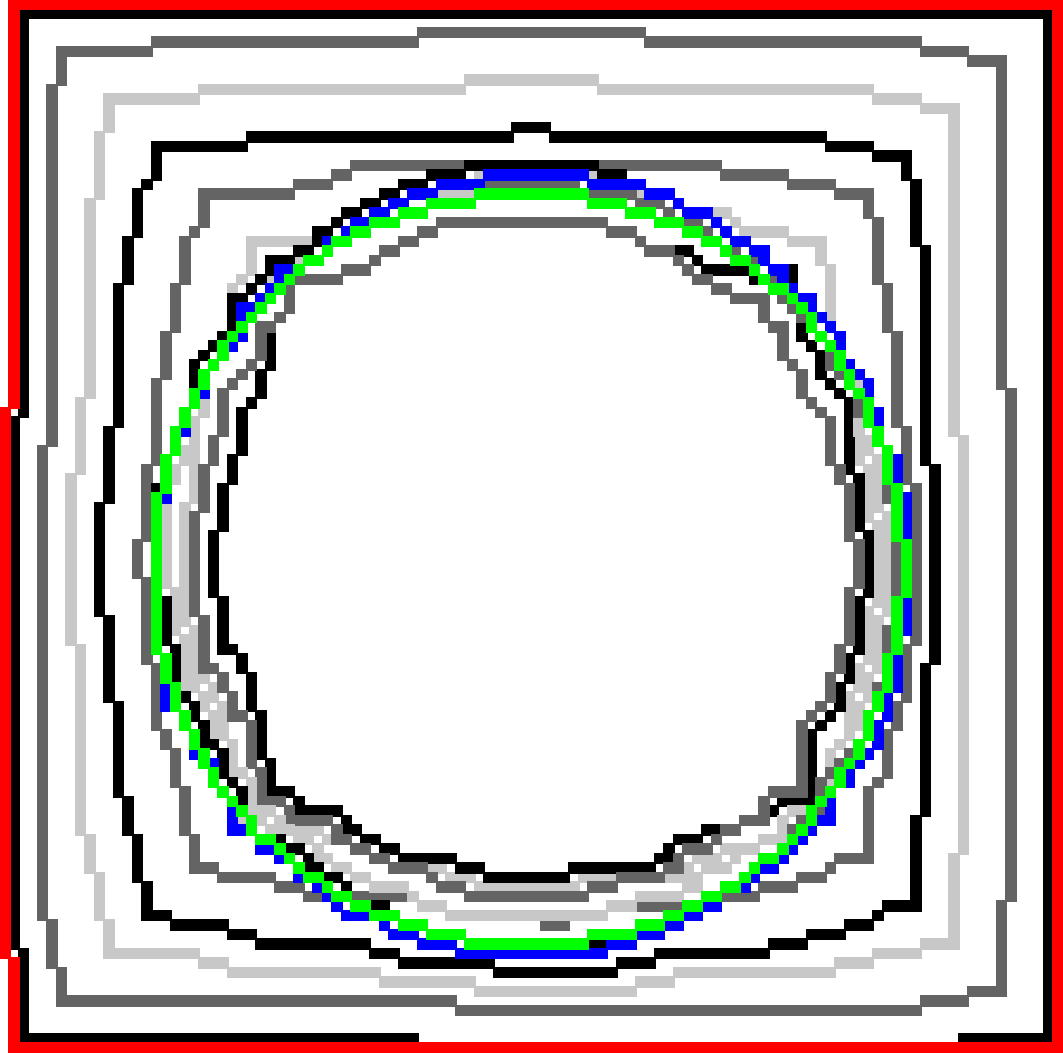
\includegraphics[scale=0.25]{figures/chapter5/flow/square/radius_5/ii/selastica/len_pen_0.01000/jonctions_1/curve_segs_4/best/gs_0.25000/summary.pdf} &
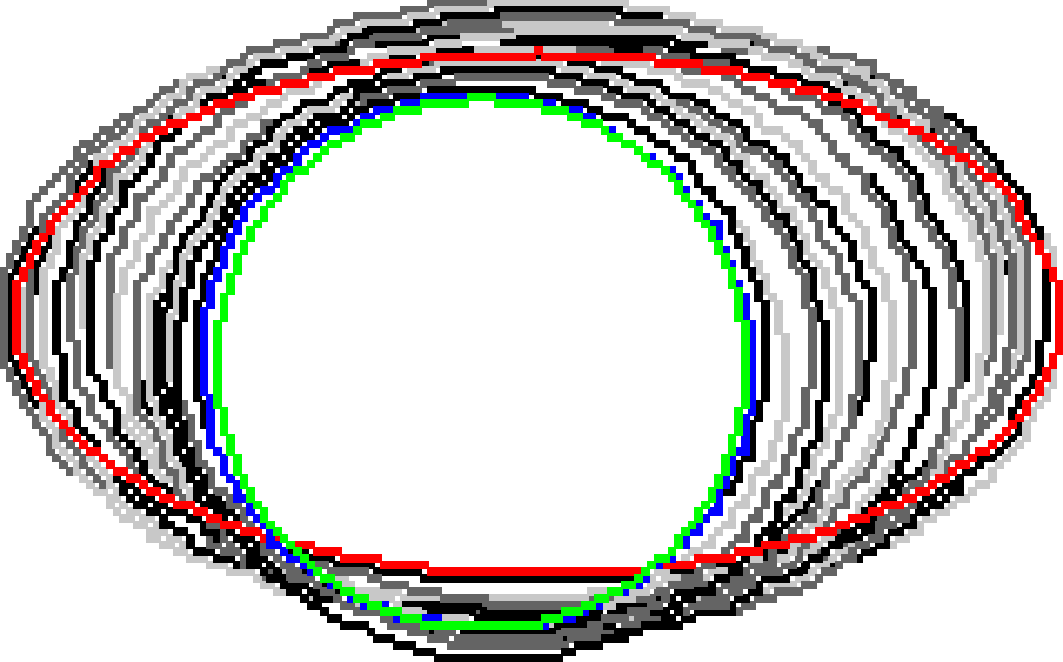
\includegraphics[scale=0.25]{figures/chapter5/flow/ellipse/radius_5/ii/selastica/len_pen_0.01000/jonctions_1/curve_segs_4/best/gs_0.25000/summary.pdf}\\[2em]
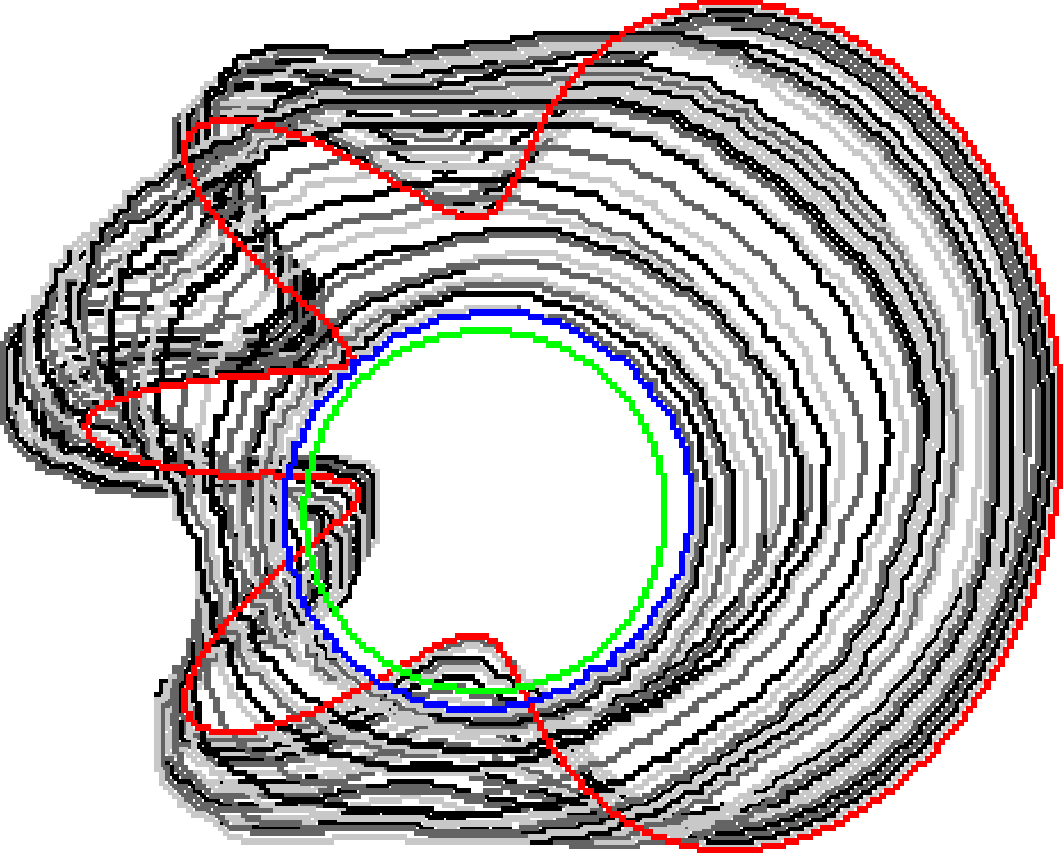
\includegraphics[scale=0.25]{figures/chapter5/flow/flower/radius_5/ii/selastica/len_pen_0.01000/jonctions_1/curve_segs_4/best/gs_0.25000/summary.pdf} &
\includegraphics[scale=0.25]{figures/chapter5/flow/bean/radius_5/ii/selastica/len_pen_0.01000/jonctions_1/curve_segs_4/best/gs_0.25000/summary.pdf} &
\includegraphics[scale=0.25]{figures/chapter5/fixed-pixels/selastica/len_pen_0.01/flower-1/summary.pdf}\\[2em]
\includegraphics[scale=0.25]{figures/chapter5/fixed-pixels/selastica/len_pen_0.01/flower-2/summary.pdf} &
\includegraphics[scale=0.25]{figures/chapter5/fixed-orientations/selastica/len_pen_0.01/curve-2/summary.pdf} &
\includegraphics[scale=0.25]{figures/chapter5/fixed-orientations/selastica/len_pen_0.01/curve-3/summary.pdf}
\end{tabular}
\caption{\daniel{\textbf{Simplified elastica results for $\mathbf{(\alpha=0.01, \beta=1)}$}.} Experiments of~\cref{ch5:sec:local-combinatorial-scheme} for the simplified digital elastica.}
\label{fig:simplified-elastica}
\end{figure}


\subsection{Optimization model for simplified digital elastica}
\label{ch5:subsec:optimization-model-simplified-digital-elastica}

In contrast with the previous section, the model described here is designed for the integral invariant estimator only. Let $\Ds \subset \frac{1}{2}\mathbb{Z}^2$ be the digitization of some shape $S \subset \mathbb{R}^2$ %using grid step $h$
 in half-integer coordinates space. We assume that $\Ds$ has $m$ pixels (located at integer coordinates) and $n$ linels (one and only one of its coordinates is $\frac{1}{2}$). Optimization variables are represented as column vectors $\vec{x} \in \daniel{\{0,1\}}^{m},\, \vec{y} \in \daniel{\{0,1\}}^{n}$ and its $i$-th coefficients are denoted  $\vec{x}_i,\vec{y}_i$.  Further, let $\vec{A} \in \daniel{\{0,1\}}^{m\times n}$ the matrix defined as
\begin{align*}
	\vec{A}_{i,j} = \left\{ \begin{array}{ll}
		1,\; \vec{x}_j \in B_{r}(\vec{y}_i)\\
		0,\; \text{otherwise}.
	\end{array}\right.
\end{align*}
%
In other words, the column vector $\vec{A}_i$ represents the pixels that are in the interior of the disk $B_{r}(y_i)$ of radius $r$ centered at $\vec{y}_i$. 
\begin{align}
	E_{\Theta}^{simp}(\vec{x},\vec{y}) =& \sum_{\vec{y}_i \in \vec{y}}{ \vec{y}_i \left(\; \alpha + \beta \hat{\kappa}_{r}^2(D,\vec{y}_i) \; \right)}\\\nonumber
			   =& \sum_{\vec{y}_i \in \vec{y}}{ \vec{y}_i \left(\; \alpha  + \beta \big( \frac{3}{r^3}(\frac{\pi}{r^2} - |B_r(\vec{y}_i)|)\big)^2\right)}\\\nonumber
			   =& \sum_{\vec{y}_i \in \vec{y}}{ \vec{y}_i \left(\; \alpha + \frac{9}{r^6}\beta \big(c^2 - 2c\vec{A}_i^T\vec{x} + \vec{x}^T\vec{A}_i\vec{A}_i^T\vec{x}\big)\right)},			   
	\end{align}
%	
where $c =  \pi r^2/2$. We remark that linels and pixels in the solution must be topologically consistent, .i.e., linels must form connected closed curves and the pixels must lie in the interior of those curves. This restriction is encoded in a set of topological constraints $T(\vec{x},\vec{y})$ detailed later. So far we have
\begin{align*}
	\min_{\vec{x} \in \daniel{\{0,1\}}^{|X|}, \vec{y} \in \daniel{\{0,1\}}^{|Y|}}{E_{\Theta}^{simp}(\vec{x},\vec{y})}, \quad \text{subject to } T(\vec{x},\vec{y}). \quad (P0)
\end{align*}
%
Additionaly, in real applications involving the minimization of elastica, we have a set of constraints $R$ that plays the role of regularization. For example, we may force some of the pixels in the original shape to be part of the solution; for imaging problems, we may add a data attachment term, and so on. Finally, we can write the general optimization problem as
\begin{align*}
	\min_{\vec{x} \in \daniel{\{0,1\}}^{|X|}, \vec{y} \in \daniel{\{0,1\}}^{|Y|}}{E_{\Theta}^{simp}(\vec{x},\vec{y})}, \quad \text{subject to } T(\vec{x},\vec{y}), R(\vec{x}) \quad (P1)
\end{align*}
%
	Formulation $P1$ is a constrained binary non-convex third order problem and likely difficult to be solved optimally. Nonetheless, we can use standard optimization techniques to acquire some intuition on the model. 	
	
\subsection{Topological constraints}
\label{ch5:subsec:topological-constraints}

The estimation ball should be applied in the \daniel{digital contour} of the shape, which oblige us to impose topological constraints in the model to avoid inconsistent solutions. In order to accomplish that, we set an arbitrary orientation for the faces and another for the edges. We choose counter-clockwise for faces; left-to-right for horizontal edges; and bottom-to-up for vertical edges. \daniel{The topological constraints are essentially the same as those implemented in the linear programming model of~\cite{schoenemann09linear} and described in~\cref{ch3:sec:discrete-methods-squared-curvature}.}


We create the vector $\vec{z} \in \daniel{\{0,1\}}^{2n}$. We map each linel identified by variable $\vec{y}_i$ to components $\vec{z}_{2i},\vec{z}_{2i+1}$, one for each possible orientation the linel may assume. Next, we extend the linel incidence matrix defined in~\cref{app2:pixel-incidence-matrix} to hold incidence with respect to oriented edges. The new matrix $\vec{T} \in \daniel{\{0,1\}}^{n \times m + 2n}$ is defined as
\begin{align*}
	0 \leq j < m, \quad \vec{T}_{i,j} = \left\{ \begin{array}{ll}
	1,& \text{Pixel $j$ is positively incident to linel $i$}\\
	-1,& \text{Pixel $j$ is negatively incident to linel $i$}\\	
	0,& \text{otherwise},
	\end{array}\right.\\[1em]
	m \leq j < m + 2n, \quad \vec{T}_{i,j} = \left\{ \begin{array}{ll}
	1,& \text{Edge $j$ is positively incident to linel $i$}\\
	-1,& \text{Edge $j$ is negatively incident to linel $i$}\\	
	0,& \text{otherwise}.
	\end{array}\right.
\end{align*}
%
Rewriting formulation (P1)
%
\begin{align*}
\begin{array}{ll}
& \displaystyle	\min \sum_{z_i \in \vec{z}}{ \vec{z}_i \left(\; \alpha + \frac{9}{r^6}\beta \big(c^2 - 2c\vec{A}_i^T\vec{x} + \vec{x}^T\vec{A}_i\vec{A}_i^T\vec{x}\big)\right)} \\
\text{subject to}\\
&	\vec{T} \times  \left[ \begin{array}{c}
							\vec{x} \\ 
							\vec{z} 
						   \end{array} \right] = 0 \\
&   R(\vec{x}),\\
&   \vec{x} \in \daniel{\{0,1\}}^{m}, \vec{z} \in \daniel{\{0,1\}}^{2n}.
\end{array}
\end{align*}
%
%
We observe that for a linel identified by variable $\vec{y}_i$, constraints $\vec{T}$ forces at most one of the variables $\vec{z}_{2i},\vec{z}_{2i+1}$ to be evaluated to one. 


\subsection{Linear relaxation of $P1$}
\label{ch5:subsec:linear-relaxation}

	The simplest model we can derive from (P1) consists in the relaxation of the optimization variables, i.e., we impose $\vec{x} \in \daniel{[0,1]}^m$ and $\vec{z} \in \daniel{[0,1]}^{2n}$, and we linearize all second and third order terms. 
	
	Consider the summation in (P1). An opt-term is an ordered sequence of optimization variables, e.g., the opt-term $\vec{z}_1\vec{x}_2\vec{x}_4$ is encoded as the sequence $(\vec{z}_1,\vec{x}_2,\vec{x}_4)$. Let $\mathcal{T}$ the collection of opt-terms of order two or higher in (P1). To linearize (P1), we associate a variable $\vec{u_i} \in \daniel{[0,1]}$ for each \daniel{$\mathcal{T}_i \in \mathcal{T}$} and we enforce $|\mathcal{T}_i|+1$ new constraints. In other words, we add the following set of linearization constraints.
\begin{align*}
	L(\vec{u}) = \left\{ \Big\{ \vec{u}_i \leq t, \quad \forall t \in \mathcal{T}_i \Big\} \cup \Big\{ \vec{u}_i \geq \displaystyle \sum_{t \in \mathcal{T}_i}{t} - |\mathcal{T}_i| + 1 \Big\} \; \Big| \; \forall \mathcal{T}_i \in \mathcal{T} \right\}
\end{align*}
%
%
\daniel{
For example, let $\vec{u}_i$ be the auxiliar variable associated with the opt-term $\vec{z}_1\vec{x}_2{x}_4$. Then, we are going to add the following constraints
\begin{align*}
	\vec{u}_i &\leq \vec{z}_1 \\
	\vec{u}_i &\leq \vec{x}_2 \\
	\vec{u}_i &\leq \vec{x}_4 \\	
	\vec{u}_i &\geq \vec{z}_1 + \vec{x}_2 + \vec{x}_4 -2.
\end{align*}}
%
The linearization of (P1) is written as
\begin{align*}
\begin{array}{ll}
& \displaystyle	\min \sum_{z_i \in \vec{z}}{ \vec{z}_i \left(\; \alpha + \frac{9}{r^6}\beta \big(c^2 - 2c\vec{A}_i^T\vec{x} + \vec{x}^T\vec{A}_i\vec{A}_i^T\vec{x}\big)\right)} \\
\text{subject to}\\
&	\vec{T} \times  \left[ \begin{array}{c}
							\vec{x} \\ 
							\vec{z} 
						   \end{array} \right] = 0 \\
&   R(\vec{x}),\\
&   L(\vec{u}),\\
&   \vec{x} \in \daniel{[0,1]}^{m}, \vec{z} \in \daniel{[0,1]}^{2n}, \vec{u} \in \daniel{[0,1]}^{|\mathcal{T}|} 
\end{array}
\end{align*}
%
	Finally, to obtain a binary vector we round the partial solution vector $\vec{x^{\star}} \in \mathbb{U}^m$. For an instance with $m$ pixels we have about $2m$ linels. After linearization, we can expect to have up to $O(m^3)$ variables, dampening our attempts to solve it globally even for low resolution images. One can also try quadratic formulations by linearizing only the third order terms. Unfortunately, the matrix of quadratic terms is not semi-definite positive, fundamental condition for efficient optimization of the model.
	


\subsection{Unconstrained version of P1}
\label{ch5:subsec:unconstrained-version}

We can use the pixel incidence matrix defined in~\cref{app2:pixel-incidence-matrix} to define an unconstrained version of P1. The pixel incidence vector $\vec{q} \in \mathbb{Z}^m$ for pixels $\vec{x} \in \mathbb{B}^{m}$ is 
	\begin{align*}
		\vec{q} &= \vec{P}^T\vec{P} \vec{x}
	\end{align*}
%
In order to supress the sign, we define diagonal matrix $\vec{Q} \in \mathbb{R}^{m \times m }$ as
\begin{align*}
	\vec{Q} = diag(\vec{q})diag(\vec{q})
\end{align*}
%
Let $\vec{B} \in \mathbb{B}^{m\times m}$ such that column vector $\vec{B}_j$ represents the pixels in the interior of a disk of radius $R$ centered at pixel $i$. Finally, we search for solutions of
\begin{align}
	\min_{\vec{x}} \frac{9}{R^6}\sum_{j}^{m}{\left( \frac{\pi R^2}{2} - \frac{1}{2}\boldsymbol{\mathbf{1}}^T{\vec{Q}}\vec{B}_j \right)^2},
	\label{eq:unconstrained-digital-elastica}
\end{align}
%
%
where $\mathbf{1} = (1,1, \cdots , 1)^T \in \mathbb{R}^m$. ~\cref{eq:unconstrained-digital-elastica} involves the minimization of a fourth order equation and therefore hard to be optimized.

\section{Conclusion}
\label{ch5:sec:conclusion}
\daniel{
We have defined a local combinatorial scheme and provided an algorithm to minimize the digital elastica. We have shown experimental results of the LocalSearch algorithm for shapes with different geometries and we observed that the method converges to the expected global optimum in the free elastica problem, justifying the interest for multigrid convergent estimators. The same model can also be used to solve the constrained elastica problem, but its more likely to stop in a local minimum. 

We observed that a global optimization method is important to recover the completion property of curvature. However, the high order of the elastica energy makes it a challenging energy to be globally optimized. We sketched some global optimization models for minimizing the simplified elastica (of lower order) using standard techniques of optimization. The difficulties we pointed out suggest that a practical global optimization model using the II estimator, if it exists, should make use of ingenious techniques. 

Nonetheless, we believe it is still possible to partially recover the completion effect based on local approaches, more likely to have practical implementations. In the next chapter, we describe a second local model faster than the one proposed in this chapter.
}

%We gave a historical review of the elastica and we defined the digital elastica energy in~\cref{ch5:sec:continuous-digital-elastica}. The local combinatorial scheme defined in~\cref{ch5:sec:local-combinatorial-scheme} can evolve different shapes guided by the minimization of digital elastica energy and it eventually reaches global optimum in the free elastica problem, justifying the interest for multigrid convergent estimators. The model can also be used to solve the constrained elastica problem, but its more likely to stop in a local minimum. Finnaly, we sketch some global optimization models in~\cref{ch5:sec:global-optimization} for minimizing the simplified elastica using standard techniques of optimization. The difficulties we pointed out suggest that a practical global optimization model is unlikely to exist. In the next chapter we explore a model that decreases the elastica energy and that can be used in practice.

